\chapter{Results and Operational Robustness Analysis}
\label{chap:results}

Il presente capitolo espone i risultati sperimentali della pipeline di valutazione
\textsc{FAIR-Lab}, con particolare attenzione alla robustezza operativa di sistemi
di classificazione automatizzata di immagini basati su \gls{ai} in uno scenario di
triage forense digitale. L'obiettivo dell'analisi non è ordinare i modelli
esclusivamente in base alla loro accuratezza nominale, bensì valutare se gli
output prodotti rimangano affidabili in presenza di input puliti, campioni
out-of-distribution, trasformazioni anti-forensi e perturbazioni adversariali. In
questa prospettiva, assumono particolare rilievo i falsi negativi relativi alla
classe \texttt{weapon}, le predizioni ad alta confidenza su campioni fuori
distribuzione e i requisiti di tracciabilità necessari per confrontare modelli
proxy trasparenti con strumenti forensi commerciali operanti come sistemi
black-box \cite{costantini2019digital,sanna2024preliminary,sanna2025pixelperfect}.

Nel corso del capitolo viene mantenuta una distinzione metodologica esplicita
tra i modelli proxy trasparenti, per i quali risultano disponibili architetture,
checkpoint, rappresentazioni intermedie e output predittivi, e gli strumenti
forensi commerciali, che operano come sistemi black-box o quasi black-box, poiché
la loro logica interna di classificazione è proprietaria e non direttamente
ispezionabile. Tale distinzione non è soltanto tecnica, ma incide direttamente
sulla tracciabilità, sull'auditabilità e sull'interpretazione probatoria degli
output assistiti da \gls{ai} all'interno di workflow forensi
\cite{iso27041,iso27042,swgde2014validation}.

L'organizzazione del capitolo segue la sequenza operativa attesa delle diverse
condizioni sperimentali in un contesto investigativo. Le prestazioni su input
puliti definiscono la baseline di riferimento; il comportamento su campioni
out-of-distribution e su trasformazioni anti-forensi rappresenta condizioni
realistiche che possono emergere nel corso di indagini digitali; le perturbazioni
adversariali descrivono invece tentativi deliberati di evasione e costituiscono
la condizione di stress più severa considerata in questa valutazione
\cite{hendrycks2017baseline,hendrycks2019benchmarking,biggio2018wild}. La
valutazione degli strumenti forensi commerciali è trattata come livello
black-box distinto, introdotto dopo la presentazione dei risultati controllati dei
modelli proxy e dopo la definizione del forensic evaluation bundle.

% ─────────────────────────────────────────────────────────────────────────────
\section{Experimental Evaluation Status and Dataset Overview}
\label{sec:results-status}
% ─────────────────────────────────────────────────────────────────────────────

La valutazione sperimentale si basa sugli artefatti generati attraverso la
metodologia descritta nel Capitolo~\ref{chap:methodology}. Allo stato attuale,
risultano completate la costruzione del dataset, il congelamento semantico delle
classi, la generazione degli split, l'addestramento dei modelli proxy, la
generazione delle perturbazioni, la valutazione dei modelli proxy e la
costruzione del forensic evaluation bundle. La valutazione black-box degli
strumenti forensi commerciali è invece considerata una fase operativa separata,
poiché dipende dalla disponibilità dei tool, dai moduli effettivamente abilitati,
dai formati di esportazione e dalla successiva normalizzazione degli output
proprietari \cite{sanna2024preliminary,sanna2025pixelperfect,magnet,xways,cellebrite,oxygen}.

Questa separazione è metodologicamente rilevante. Il livello dei modelli proxy
fornisce una baseline trasparente e riproducibile, poiché architetture,
checkpoint, fold di addestramento, predizioni e metriche sono disponibili per
ispezione e verifica. Il livello degli strumenti forensi commerciali riflette
invece una condizione operativa differente: l'analista interagisce con strumenti
professionali la cui logica interna di classificazione non è pienamente
accessibile, e la valutazione deve quindi basarsi sugli output osservabili, sulle
categorie esportate, sui tag assegnati, sugli eventuali valori di confidenza e
sul matching hash-based rispetto alla ground truth sperimentale
\cite{casey2011digital,nist2006guide,iso27041,iso27042}.

La Tabella~\ref{tab:results-evaluation-status} riporta lo stato corrente delle
principali componenti sperimentali, fornendo una sintesi audit-ready del workflow
di valutazione al momento della redazione.

\begin{table}[H]
\centering
\scriptsize
\renewcommand{\arraystretch}{1.15}
\setlength{\tabcolsep}{4pt}
\caption{Stato corrente del workflow di valutazione sperimentale.}
\label{tab:results-evaluation-status}
\begin{tabularx}{\textwidth}{@{}p{0.28\textwidth} p{0.22\textwidth} X@{}}
\toprule
\textbf{Componente} & \textbf{Stato} & \textbf{Sintesi operativa} \\
\midrule

Dataset finale &
\textbf{Congelato} &
1500 immagini bilanciate: 500 \texttt{weapon}, 500 \texttt{non\_weapon} e 500 \texttt{ood}. \\

Subset binario &
\textbf{Congelato} &
1000 immagini: 500 \texttt{weapon} e 500 \texttt{non\_weapon}; usato per clean, adversarial e anti-forensic evaluation. \\

Split clean e OOD &
\textbf{Completati} &
Cinque fold binari clean e un insieme \gls{ood} separato, derivati dai manifest congelati. \\

Addestramento proxy &
\textbf{Completato} &
Checkpoint fold-aware prodotti per \texttt{efficientnet\_b0}, \texttt{resnet18} e \texttt{clip}. \\

Valutazione proxy &
\textbf{Completata} &
Valutazione su input clean, \gls{ood}, adversariali e anti-forensi. \\

Attacchi adversariali &
\textbf{Generati} &
\texttt{fgsm}, \texttt{superdeepfool}, \texttt{sigma\_zero}, \texttt{one\_pixel}, \texttt{color\_shift}. \\

Trasformazioni anti-forensi &
\textbf{Generate} &
\texttt{jpeg\_recompression}, \texttt{resample\_resize}, \texttt{gaussian\_blur}, \texttt{histogram\_modification}, \texttt{contrast\_stretching}. \\

Forensic evaluation bundle &
\textbf{Generato} &
11\,500 file predisposti per la valutazione black-box dei tool forensi. \\

Magnet AXIOM / Magnet.AI &
\textbf{Consolidato} &
Bundle processato ed export normalizzato; \texttt{Possible weapons} ricondotto alla predizione positiva \texttt{weapon}. \\

X-Ways / Excire Photo AI &
\textbf{Consolidato} &
Valutato come semantic retrieval black-box con tre configurazioni: \texttt{D20}, \texttt{D50}, \texttt{D80}. \\

Cellebrite UFED &
\textbf{Fuori confronto quantitativo} &
Rilevante nella pipeline operativo-forense, ma privo di export normalizzati comparabili per il bundle. \\

Oxygen Forensic Detective &
\textbf{Fuori confronto quantitativo} &
Non incluso nella comparazione quantitativa per assenza di output strutturati e direttamente mappabili alla ground truth. \\

Explainability &
\textbf{Integrata} &
Casi rappresentativi generati con \gls{ig}; analisi qualitativa e diagnostica, non metrica primaria. \\

\bottomrule
\end{tabularx}
\end{table}

Il corpus sperimentale risultante è organizzato in condizioni clean,
out-of-distribution, adversariali e anti-forensi. I campioni binari clean e
perturbati derivano dal subset ufficiale \texttt{weapon}/\texttt{non\_weapon},
mentre i campioni OOD sono valutati separatamente e non sono utilizzati come
target degli attacchi. Tale distinzione preserva la differenza tra classificazione
binaria nominale, comportamento fuori distribuzione e robustezza rispetto a input
manipolati.

La Tabella~\ref{tab:results-corpus-composition} riporta la composizione
consolidata del corpus di valutazione utilizzato nei livelli proxy-model e
forensic-tool.

\begin{table}[H]
\centering
\caption{Composizione del corpus sperimentale e del forensic evaluation bundle.}
\label{tab:results-corpus-composition}
\begin{tabularx}{0.88\textwidth}{@{}l r X@{}}
\toprule
\textbf{Condizione} & \textbf{File} & \textbf{Ruolo nella valutazione} \\
\midrule

Clean
&
1000
&
Valutazione binaria nominale sui campioni \texttt{weapon} e
\texttt{non\_weapon}. \\

OOD
&
500
&
Insieme di valutazione out-of-distribution e borderline, mantenuto separato dal
task di classificazione binaria. \\

Adversarial
&
5000
&
Cinque famiglie di perturbazioni applicate al subset binario di 1000 immagini,
con 1000 file generati per ciascuna famiglia di perturbazione. \\

Anti-forensic
&
5000
&
Cinque trasformazioni model-agnostic applicate al subset binario di 1000
immagini, con 1000 file generati per ciascuna trasformazione. \\

\midrule
\textbf{Totale}
&
\textbf{11\,500}
&
Forensic evaluation bundle completo, predisposto per la valutazione dei modelli
proxy e per il processamento mediante strumenti forensi black-box. \\

\bottomrule
\end{tabularx}
\end{table}

Il forensic evaluation bundle costituisce il collegamento operativo tra il
livello sperimentale controllato e il livello di valutazione basato su strumenti
forensi professionali. Esso fornisce una directory di input cieca e
semanticamente neutra per i tool forensi, preservando al contempo ground truth,
informazioni di provenienza, metadati sulle perturbazioni e mapping hash-based in
file separati. In termini operativi, gli strumenti forensi devono processare
soltanto la directory cieca di input, mentre il livello dei metadati è riservato
alle fasi successive di matching, normalizzazione e audit degli export.

Questo disegno riduce il rischio di bias indotto dai path o dall'analista, poiché
i tool non sono esposti a label di classe, nomi degli attacchi, identificativi di
sorgente o informazioni sui fold durante l'importazione. Al tempo stesso, la
presenza di mapping SHA256 e MD5 consente di ricondurre ciascun risultato
esportato al corrispondente artefatto sperimentale. Tale requisito di
tracciabilità è centrale per l'interpretazione forense dei risultati, poiché
permette di distinguere tra errori di classificazione, file non supportati,
mancate rilevazioni, output non categorizzati e limitazioni specifiche del formato
di export del singolo tool \cite{casey2011digital,nist2006guide,iso27041,iso27042,swgde2014validation}.

Le sezioni successive presentano i risultati quantitativi, a partire dalla
baseline clean descritta nella Sezione~\ref{sec:results-clean-baseline}.

% ─────────────────────────────────────────────────────────────────────────────
\section{Clean Baseline Performance}
\label{sec:results-clean-baseline}
% ─────────────────────────────────────────────────────────────────────────────

La valutazione su input clean costituisce la baseline sperimentale rispetto alla
quale interpretare il comportamento dei modelli nelle condizioni successive,
ossia campioni \gls{ood}, trasformazioni anti-forensi e perturbazioni
adversariali. In questa fase, i modelli sono valutati sul subset binario
ufficiale composto da 1000 immagini, bilanciate tra 500 campioni
\texttt{weapon} e 500 campioni \texttt{non\_weapon}. La classe positiva è
definita come \texttt{weapon}, mentre la classe negativa è definita come
\texttt{non\_weapon}; di conseguenza, i falsi negativi indicano immagini
contenenti armi classificate come non rilevanti, mentre i falsi positivi indicano
immagini non contenenti armi classificate come \texttt{weapon}.

La Tabella~\ref{tab:results-clean-baseline-metrics} riporta le principali
metriche prestazionali dei tre modelli proxy sul subset binario clean.

\begin{table}[H]
\centering
\scriptsize
\setlength{\tabcolsep}{2.8pt}
\renewcommand{\arraystretch}{1.15}
\caption{Prestazioni clean dei modelli proxy sul subset binario.}
\label{tab:results-clean-baseline-metrics}
\begin{tabularx}{\textwidth}{@{}l *{10}{>{\centering\arraybackslash}X}@{}}
\toprule
\textbf{Modello} &
\textbf{Acc.} &
\textbf{Bal.} &
\textbf{M-P} &
\textbf{M-R} &
\textbf{M-F1} &
\textbf{P\textsubscript{w}} &
\textbf{R\textsubscript{w}} &
\textbf{F1\textsubscript{w}} &
\textbf{\acrshort{fpr}} &
\textbf{\acrshort{fnr}} \\
\midrule
EfficientNet-B0 & 0.978 & 0.978 & 0.978 & 0.978 & 0.978 & 0.972 & 0.984 & 0.978 & 0.028 & 0.016 \\
ResNet18        & 0.964 & 0.964 & 0.964 & 0.964 & 0.964 & 0.958 & 0.970 & 0.964 & 0.042 & 0.030 \\
\acrshort{clip} & 0.927 & 0.927 & 0.933 & 0.927 & 0.927 & 0.881 & 0.988 & 0.931 & 0.134 & 0.012 \\
\bottomrule
\end{tabularx}

\vspace{0.4em}
\footnotesize
\textit{Nota.} \textit{Bal.} indica la balanced accuracy; \textit{M-P},
\textit{M-R} e \textit{M-F1} indicano rispettivamente macro-precision,
macro-recall e macro-F1; \(P_w\), \(R_w\) e \(F1_w\) indicano precision,
recall e F1-score per la classe \texttt{weapon}.
\end{table}

EfficientNet-B0 ottiene la prestazione nominale più elevata, con accuracy pari a
0.978 e macro-F1 pari a 0.978. ResNet18 mostra una prestazione leggermente
inferiore ma ancora elevata, con accuracy pari a 0.964. \gls{clip} ottiene
un'accuracy pari a 0.927, mostrando una dinamica diversa rispetto ai due modelli
supervisionati: il recall sulla classe \texttt{weapon} è molto alto, pari a
0.988, ma il valore di \gls{fpr} risulta sensibilmente superiore, pari a 0.134.
Questo comportamento suggerisce che \gls{clip} tende a privilegiare una maggiore
sensibilità verso la classe \texttt{weapon}, al costo di un numero più elevato di
falsi positivi sulla classe \texttt{non\_weapon}.

La Tabella~\ref{tab:results-clean-confusion-matrices} riporta le confusion
matrix aggregate per modello, utilizzando il layout\\
\(\left[\left[\gls{tn}, \gls{fp}\right], \left[\gls{fn}, \gls{tp}\right]\right]\).

\begin{table}[H]
\centering
\caption{Confusion matrix clean dei modelli proxy.}
\label{tab:results-clean-confusion-matrices}
\begin{tabular}{@{}l r r r r@{}}
\toprule
\textbf{Modello} & \textbf{\gls{tn}} & \textbf{\gls{fp}} & \textbf{\gls{fn}} & \textbf{\gls{tp}} \\
\midrule
EfficientNet-B0 & 486 & 14 & 8  & 492 \\
ResNet18        & 479 & 21 & 15 & 485 \\
\gls{clip}      & 433 & 67 & 6  & 494 \\
\bottomrule
\end{tabular}
\end{table}

La stessa distribuzione degli errori è visualizzata nella
Figura~\ref{fig:results-clean-confusion-matrices}, che rende evidente il diverso
profilo operativo dei tre modelli: EfficientNet-B0 minimizza il numero totale di
errori, ResNet18 mantiene un comportamento intermedio, mentre \gls{clip} riduce
i falsi negativi sulla classe \texttt{weapon} al costo di un numero più elevato
di falsi positivi.

\begin{figure}[htbp]
\centering

\begin{minipage}{0.48\textwidth}
\centering
\small EfficientNet-B0

\vspace{0.2em}
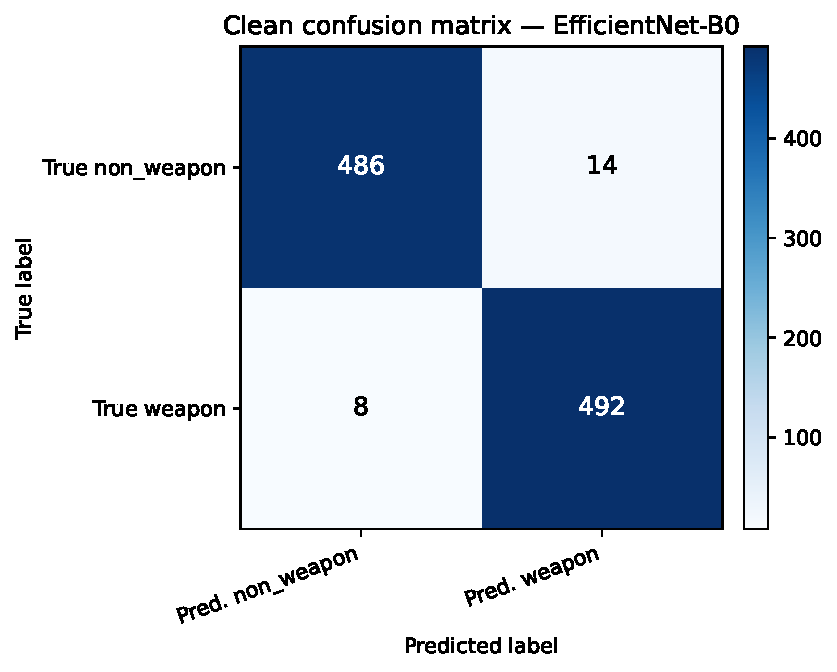
\includegraphics[width=\linewidth]{images/fig_clean_confusion_matrix_efficientnet_b0.pdf}
\end{minipage}
\hfill
\begin{minipage}{0.48\textwidth}
\centering
\small ResNet18

\vspace{0.2em}
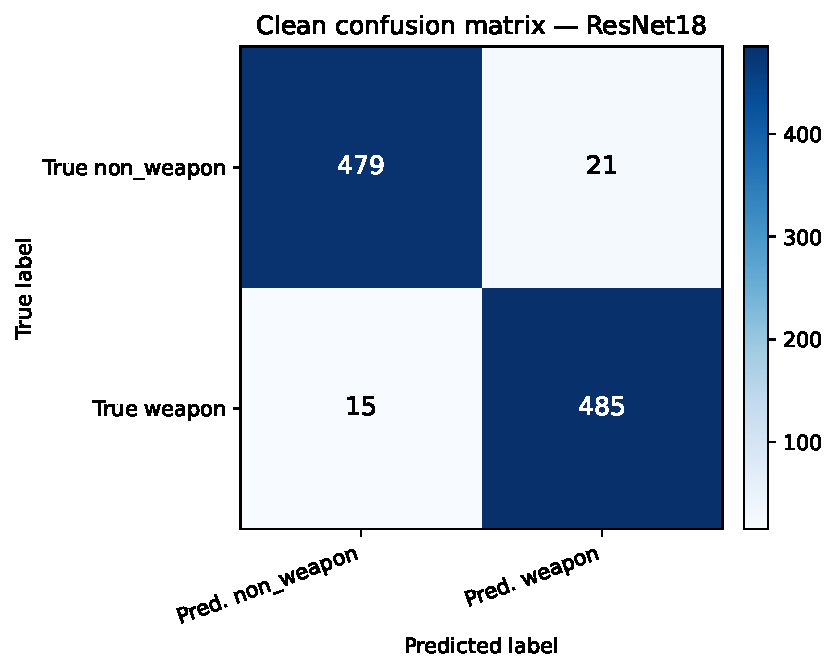
\includegraphics[width=\linewidth]{images/fig_clean_confusion_matrix_resnet18.pdf}
\end{minipage}

\vspace{0.8em}

\begin{minipage}{0.48\textwidth}
\centering
\small \acrshort{clip}

\vspace{0.2em}
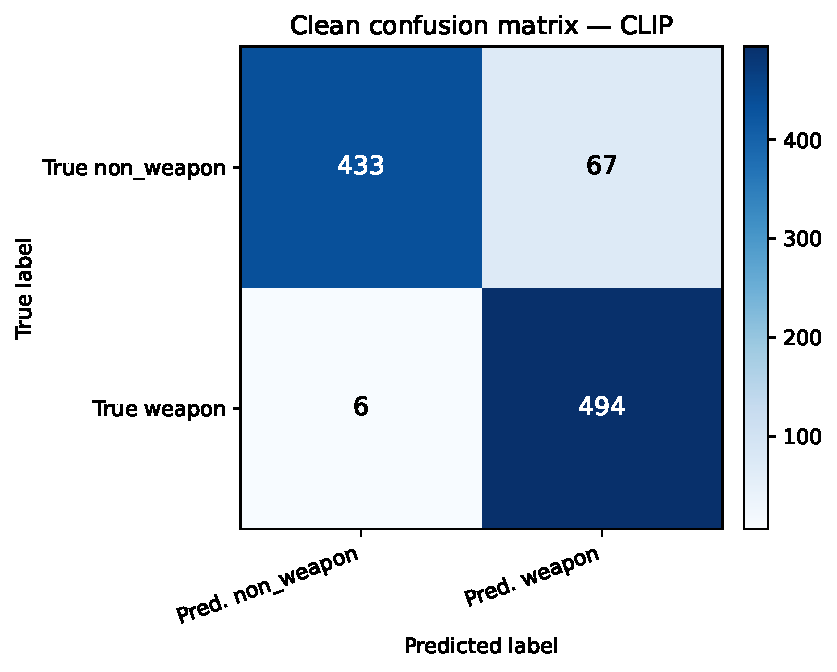
\includegraphics[width=\linewidth]{images/fig_clean_confusion_matrix_clip.pdf}
\end{minipage}

\caption{Confusion matrix clean dei tre modelli proxy sul subset binario. Le righe rappresentano la label reale, mentre le colonne rappresentano la label predetta.}
\label{fig:results-clean-confusion-matrices}
\end{figure}



Dal punto di vista forense, il dato più critico è rappresentato dai falsi
negativi sulla classe \texttt{weapon}. EfficientNet-B0 produce 8 falsi negativi,
ResNet18 ne produce 15, mentre \gls{clip} ne produce 6. Tuttavia, \gls{clip}
produce anche 67 falsi positivi, valore sensibilmente più alto rispetto ai 14 di
EfficientNet-B0 e ai 21 di ResNet18. Ne deriva che il confronto clean non può
essere letto soltanto in termini di accuracy complessiva, ma deve considerare il
diverso bilanciamento tra sensibilità verso le armi e rischio di segnalazioni
improprie.

Nel complesso, la baseline clean conferma che i modelli proxy sono in grado di
raggiungere prestazioni elevate in condizioni nominali. Tuttavia, la differenza
tra accuracy, \gls{fpr} e \gls{fnr} evidenzia già in assenza di perturbazioni un
aspetto rilevante per il triage forense: modelli con accuracy simile possono
produrre profili di rischio operativo diversi, soprattutto quando l'errore
riguarda la mancata segnalazione di contenuti \texttt{weapon} oppure la
classificazione impropria di contenuti \texttt{non\_weapon} come potenzialmente
rilevanti.

% ─────────────────────────────────────────────────────────────────────────────
\section{Out-of-Distribution Behavior and False Positive Risk}
\label{sec:results-ood}
% ─────────────────────────────────────────────────────────────────────────────

La valutazione \gls{ood} analizza il comportamento dei modelli proxy su immagini
che non appartengono al task binario nominale \texttt{weapon}/\texttt{non\_weapon}.
Questi campioni includono contenuti borderline o fuori distribuzione, quali
coltelli, spade, repliche, airsoft, render sintetici, immagini videoludiche,
scene di guerra, mezzi militari, esplosioni e immagini degradate o anomale. A
differenza delle perturbazioni adversariali e delle trasformazioni anti-forensi,
la condizione \gls{ood} non rappresenta un attacco, ma un rischio operativo
realistico: in un workflow investigativo, immagini ambigue o non perfettamente
aderenti alle classi del modello possono essere comunque sottoposte ad analisi
automatica \cite{hendrycks2017baseline,liang2018odin,fort2021exploring}.

Le metriche sono aggregate su 2\,500 predizioni, ottenute valutando le 500 immagini
\gls{ood} attraverso i cinque checkpoint fold-aware di ciascun modello. Questa
scelta mantiene la coerenza con la strategia di valutazione adottata per il
subset binario, pur preservando la separazione concettuale tra campioni
\gls{ood} e task \texttt{weapon}/\texttt{non\_weapon}. Il valore \emph{weapon
rate} indica la quota di campioni \gls{ood} classificati come \texttt{weapon};
il valore \emph{high-confidence rate} indica invece la quota di predizioni con
confidenza almeno pari a 0.9.


\begin{table}[H]
\centering
\scriptsize
\setlength{\tabcolsep}{4pt}
\renewcommand{\arraystretch}{1.15}
\caption{Comportamento dei modelli proxy sui campioni \gls{ood}.}
\label{tab:results-ood-behavior}
\begin{tabular}{@{}l r r r r r r@{}}
\toprule
\textbf{Modello} &
\textbf{Tot.} &
\textbf{Pred. w} &
\textbf{Pred. nw} &
\textbf{W-rate} &
\textbf{Conf.} &
\textbf{HC-rate} \\
\midrule
EfficientNet-B0 & 2\,500 & 924  & 1576 & 0.370 & 0.850 & 0.501 \\
ResNet18        & 2\,500 & 1094 & 1406 & 0.438 & 0.890 & 0.647 \\
\acrshort{clip} & 2\,500 & 2089 & 411  & 0.836 & 0.536 & 0.000 \\
\bottomrule
\end{tabular}

\vspace{0.4em}
\footnotesize
\textit{Nota.} \textit{Pred. w} indica le predizioni \texttt{weapon};
\textit{Pred. nw} indica le predizioni \texttt{non\_weapon};
\textit{W-rate} indica la quota di campioni \gls{ood} classificati come
\texttt{weapon}; \textit{Conf.} indica la confidenza media; \textit{HC-rate}
indica la quota di predizioni con confidenza almeno pari a 0.9. Il totale di 2\,500 predizioni per modello è ottenuto valutando le 500 immagini
\gls{ood} attraverso ciascuno dei cinque checkpoint fold-aware.
\end{table}


La Figura~\ref{fig:results-ood-weapon-rate-confidence} visualizza il confronto
tra weapon rate, confidenza media e high-confidence rate, mentre la
Figura~\ref{fig:results-ood-confidence-distribution} mostra la distribuzione
delle confidenze predittive sui campioni \gls{ood}.

\begin{figure}[H]
\centering

\includegraphics[width=0.88\textwidth]{images/fig_ood_weapon_rate_and_confidence.pdf}
\caption{Comportamento dei modelli proxy sui campioni \gls{ood}: quota di predizioni \texttt{weapon}, confidenza media e quota di predizioni ad alta confidenza.}
\label{fig:results-ood-weapon-rate-confidence}
\end{figure}

I risultati mostrano tre profili distinti. \gls{clip} classifica come
\texttt{weapon} una quota molto elevata di campioni \gls{ood}, pari a 0.836,
ma lo fa con una confidenza media contenuta e senza predizioni sopra la soglia
di alta confidenza. Il valore nullo di high-confidence rate per \gls{clip}
indica infatti che nessuna predizione \gls{ood} supera la soglia di confidenza
0.9, in coerenza con la minore confidenza complessiva del modello su input fuori
distribuzione. EfficientNet-B0 e ResNet18, al contrario, classificano come
\texttt{weapon} una quota inferiore di campioni \gls{ood}, rispettivamente pari
a 0.370 e 0.438, ma con confidenze medie molto più alte. In particolare,
ResNet18 presenta un high-confidence rate pari a 0.647, mentre EfficientNet-B0
raggiunge 0.501.

\begin{figure}[H]
\centering
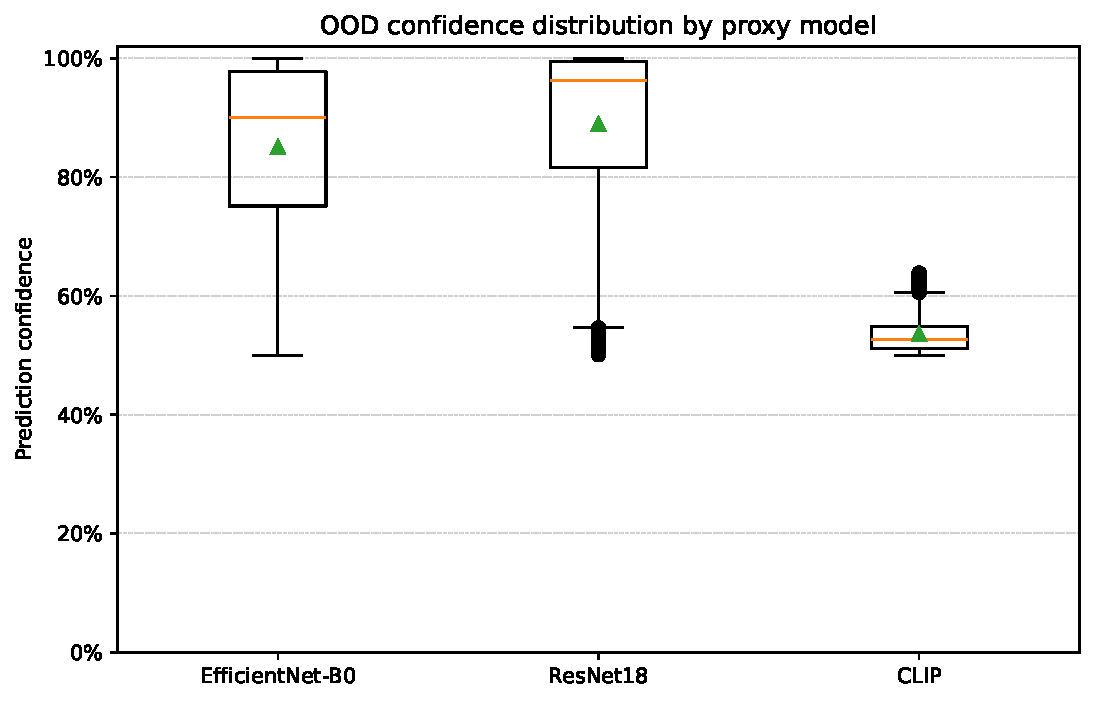
\includegraphics[width=0.82\textwidth]{images/fig_ood_confidence_distribution.pdf}
\caption{Distribuzione della confidenza predittiva sui campioni \gls{ood} per ciascun modello proxy. Il grafico evidenzia il comportamento più concentrato e meno confident di \gls{clip} rispetto ai due modelli supervisionati.}
\label{fig:results-ood-confidence-distribution}
\end{figure}

La Figura~\ref{fig:results-ood-confidence-distribution} mostra che la
distribuzione delle confidenze di \gls{clip} è più concentrata verso valori
intermedi, mentre EfficientNet-B0 e ResNet18 presentano distribuzioni più
polarizzate verso confidenze alte, confermando il diverso profilo di rischio
operativo dei tre modelli.

Dal punto di vista forense, questo risultato è rilevante perché evidenzia un
rischio diverso rispetto alla normale misclassificazione binaria. Una predizione
errata o impropria su un campione fuori distribuzione può infatti generare una
segnalazione investigativa non pienamente fondata oppure, al contrario,
rafforzare indebitamente la percezione di rilevanza di un contenuto ambiguo. Il
caso di ResNet18 ed EfficientNet-B0 mostra che un modello può produrre meno
classificazioni \texttt{weapon} su campioni \gls{ood}, ma attribuire a tali
predizioni una confidenza elevata. Il caso di \gls{clip}, invece, mostra un
comportamento opposto: maggiore propensione a classificare come \texttt{weapon},
ma con confidenza più bassa. Questa distinzione è essenziale in un contesto
forense, nel quale la confidenza del sistema non deve essere interpretata come
prova autonoma, ma come informazione ausiliaria soggetta a verifica umana
\cite{guo2017calibration,nist2023airmf}.

% ─────────────────────────────────────────────────────────────────────────────
\section{Robustness Against Anti-Forensic Transformations}
\label{sec:results-antiforensic}
% ─────────────────────────────────────────────────────────────────────────────

La valutazione contro trasformazioni anti-forensi misura la stabilità dei modelli
proxy rispetto a manipolazioni model-agnostic che possono emergere in scenari
operativi realistici. A differenza degli attacchi adversariali, tali
trasformazioni non richiedono accesso al modello target e non sono
necessariamente progettate per massimizzare l'errore di classificazione. Esse
simulano invece alterazioni comuni del contenuto visivo o del file immagine,
quali ricompressione, ridimensionamento, sfocatura, modifica della distribuzione
tonale e normalizzazione del contrasto
\cite{stamm2010anti,yaacoub2021digital,hendrycks2019benchmarking}.

La Tabella~\ref{tab:results-antiforensic-robustness} riporta, per ciascuna
trasformazione, l'accuracy perturbata e la variazione rispetto alla baseline
clean. La variazione è calcolata come
\(\Delta=\text{accuracy}_{perturbed}-\text{accuracy}_{clean}\); pertanto, valori
negativi indicano una riduzione della prestazione, mentre valori positivi
indicano un incremento rispetto alla baseline. Eventuali incrementi lievi non
devono essere interpretati come una garanzia di robustezza generale, ma come
oscillazioni compatibili con la specifica distribuzione dei campioni trasformati
e con la sensibilità del modello alla trasformazione applicata. Le variazioni di
entità inferiore a 0.005 devono essere interpretate con cautela, poiché possono
rientrare nella variabilità inter-fold osservabile in condizioni clean e non
necessariamente indicano una differenza operativamente significativa tra la
condizione originale e quella trasformata.

\begin{table}[H]
\centering
\scriptsize
\caption{Accuracy perturbata e variazione rispetto alla baseline clean sotto trasformazioni anti-forensi.}
\label{tab:results-antiforensic-robustness}
\begin{tabular}{@{}l r r r r r r@{}}
\toprule
\textbf{Trasformazione} &
\textbf{\gls{clip} acc.} & \textbf{\(\Delta\)} &
\textbf{EffNet acc.} & \textbf{\(\Delta\)} &
\textbf{ResNet acc.} & \textbf{\(\Delta\)} \\
\midrule
\gls{jpegrecompression}     & 0.925 & -0.002 & 0.976 & -0.002 & 0.964 &  0.000 \\
\gls{resampleresize}        & 0.929 & +0.002 & 0.976 & -0.002 & 0.963 & -0.001 \\
\gls{gaussianblur}          & 0.934 & +0.007 & 0.965 & -0.013 & 0.959 & -0.005 \\
\gls{histogrammodification} & 0.925 & -0.002 & 0.973 & -0.005 & 0.934 & -0.030 \\
\gls{contraststretching}    & 0.927 &  0.000 & 0.974 & -0.004 & 0.963 & -0.001 \\
\bottomrule
\end{tabular}
\end{table}

La Figura~\ref{fig:results-antiforensic-accuracy-drop-heatmap} riporta la stessa
valutazione in termini di accuracy drop, definito come
\(\text{accuracy}_{clean}-\text{accuracy}_{perturbed}\). Di conseguenza, il
segno del drop visualizzato nella heatmap è opposto rispetto alla colonna
\(\Delta\) della Tabella~\ref{tab:results-antiforensic-robustness}.

\begin{figure}[H]
\centering
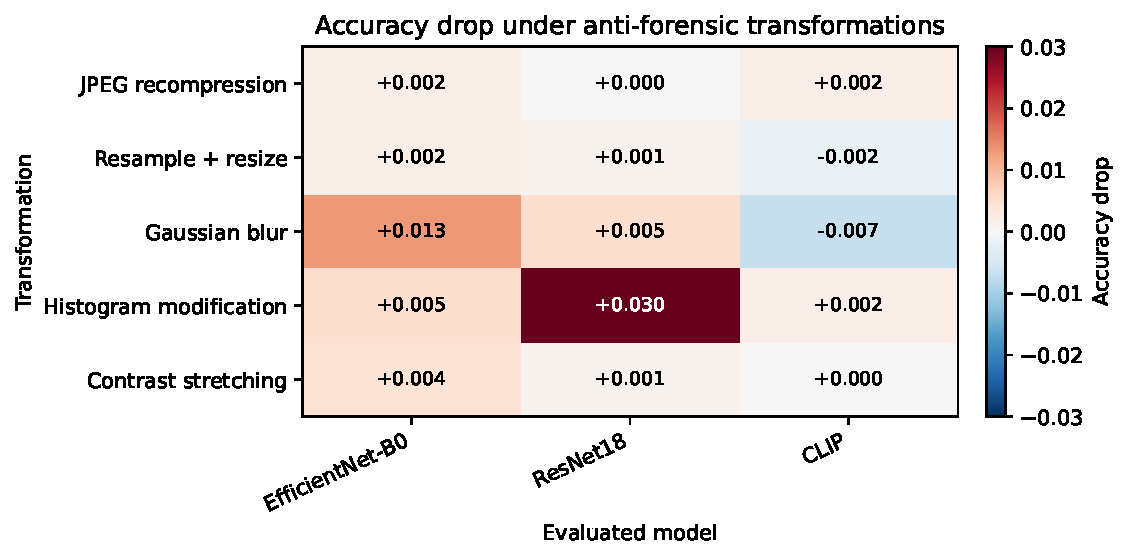
\includegraphics[width=0.88\textwidth]{images/fig_anti_forensic_accuracy_drop_heatmap.pdf}
\caption{Accuracy drop sotto trasformazioni anti-forensi. Il drop è definito come \(\text{accuracy}_{clean}-\text{accuracy}_{perturbed}\), quindi valori positivi indicano una degradazione della prestazione, mentre valori negativi indicano un lieve incremento rispetto alla baseline clean.}
\label{fig:results-antiforensic-accuracy-drop-heatmap}
\end{figure}

I risultati mostrano che le trasformazioni anti-forensi producono effetti
complessivamente contenuti; il confronto con le perturbazioni adversariali,
presentato nella sezione successiva, permette di contestualizzare questi valori
all'interno del profilo di robustezza complessivo dei modelli proxy. EfficientNet-B0 mantiene
prestazioni elevate in tutte le condizioni, ma risulta maggiormente sensibile a
\gls{gaussianblur}, con una variazione pari a -0.013. ResNet18 mostra invece la
maggiore degradazione in corrispondenza di \gls{histogrammodification}, con una
variazione pari a -0.030. \gls{clip} rimane sostanzialmente stabile, con
variazioni molto contenute e, in alcuni casi, lievi incrementi dell'accuracy.

La Figura~\ref{fig:results-antiforensic-accuracy-drop-heatmap} rende
visivamente evidente la distribuzione disomogenea degli effetti tra modelli e
trasformazioni, evidenziando in particolare l'isolamento del drop di ResNet18
sotto \gls{histogrammodification} rispetto alla generale stabilità degli altri
casi.

Dal punto di vista operativo, questi risultati non devono essere considerati
trascurabili soltanto perché i drop sono inferiori a quelli adversariali. Le
trasformazioni anti-forensi sono infatti più facilmente riconducibili a condizioni
realistiche di circolazione, compressione, modifica e ricondivisione delle
immagini. In un workflow di \gls{df}, anche una riduzione limitata della
prestazione può diventare rilevante quando riguarda contenuti investigativamente
sensibili o quando si combina con altri fattori di incertezza, quali bassa
qualità dell'immagine, contesto ambiguo o assenza di verifica manuale
sistematica.
% ─────────────────────────────────────────────────────────────────────────────
\section{Robustness Against Adversarial Perturbations}
\label{sec:results-adversarial}
% ─────────────────────────────────────────────────────────────────────────────

La valutazione adversarial misura la risposta dei modelli proxy a perturbazioni
progettate per alterare il comportamento del classificatore
\cite{szegedy2014intriguing,goodfellow2015explaining,biggio2018wild}. Nel contesto della
presente tesi, tali perturbazioni non sono analizzate come fine autonomo di
\gls{aml}, ma come stressor sperimentali utili a valutare l'affidabilità
operativa di sistemi \gls{ai}-based in scenari forensi. L'interesse principale
non riguarda quindi soltanto la capacità dell'attacco di ridurre l'accuracy, ma
il rischio che immagini della classe \texttt{weapon} vengano riclassificate come
\texttt{non\_weapon}, generando falsi negativi potenzialmente critici in un
processo di triage investigativo.

Gli attacchi model-dependent sono generati contro EfficientNet-B0. Questa scelta
riflette uno scenario white-box nel quale l'avversario dispone di accesso pieno a
un singolo modello target; la trasferibilità verso architetture differenti viene
quindi valutata empiricamente, anziché assunta a priori
\cite{biggio2018wild,nowroozi2021survey,barni2018cf}. \gls{colorshift} è
invece trattato come perturbazione model-agnostic di stile adversarial.

La Tabella~\ref{tab:results-adversarial-robustness} riporta l'accuracy
perturbata e la variazione rispetto alla baseline clean per ciascuna famiglia di
perturbazioni, includendo famiglie di attacco riconducibili a \gls{fgsm}, metodi
sparse pixel-level e varianti decision-boundary-oriented
\cite{goodfellow2015explaining,su2019onepixel,zhao2024sigmazero,zhang2024superdeepfool}. Anche in questo caso la variazione è calcolata come
\(\Delta=\text{accuracy}_{perturbed}-\text{accuracy}_{clean}\).

\begin{table}[H]
\centering
\scriptsize
\caption{Accuracy perturbata e variazione rispetto alla baseline clean sotto perturbazioni adversariali.}
\label{tab:results-adversarial-robustness}
\begin{tabular}{@{}l r r r r r r@{}}
\toprule
\textbf{Perturbazione} &
\textbf{\gls{clip} acc.} & \textbf{\(\Delta\)} &
\textbf{EffNet acc.} & \textbf{\(\Delta\)} &
\textbf{ResNet acc.} & \textbf{\(\Delta\)} \\
\midrule
\gls{fgsm}          & 0.914 & -0.013 & 0.575 & -0.403 & 0.918 & -0.046 \\
\gls{superdeepfool} & 0.926 & -0.001 & 0.931 & -0.047 & 0.964 &  0.000 \\
\gls{sigmazero}     & 0.944 & +0.017 & 0.015 & -0.963 & 0.968 & +0.004 \\
\gls{onepixel}      & 0.928 & +0.001 & 0.976 & -0.002 & 0.963 & -0.001 \\
\gls{colorshift}    & 0.925 & -0.002 & 0.977 & -0.001 & 0.963 & -0.001 \\
\bottomrule
\end{tabular}
\end{table}

La Figura~\ref{fig:results-adversarial-accuracy-drop-heatmap} riporta i medesimi
risultati in termini di accuracy drop, definito come
\(\text{accuracy}_{clean}-\text{accuracy}_{perturbed}\). Anche in questo caso,
il segno del drop visualizzato nella heatmap è opposto rispetto alla colonna
\(\Delta\) della Tabella~\ref{tab:results-adversarial-robustness}.

\begin{figure}[H]
\centering
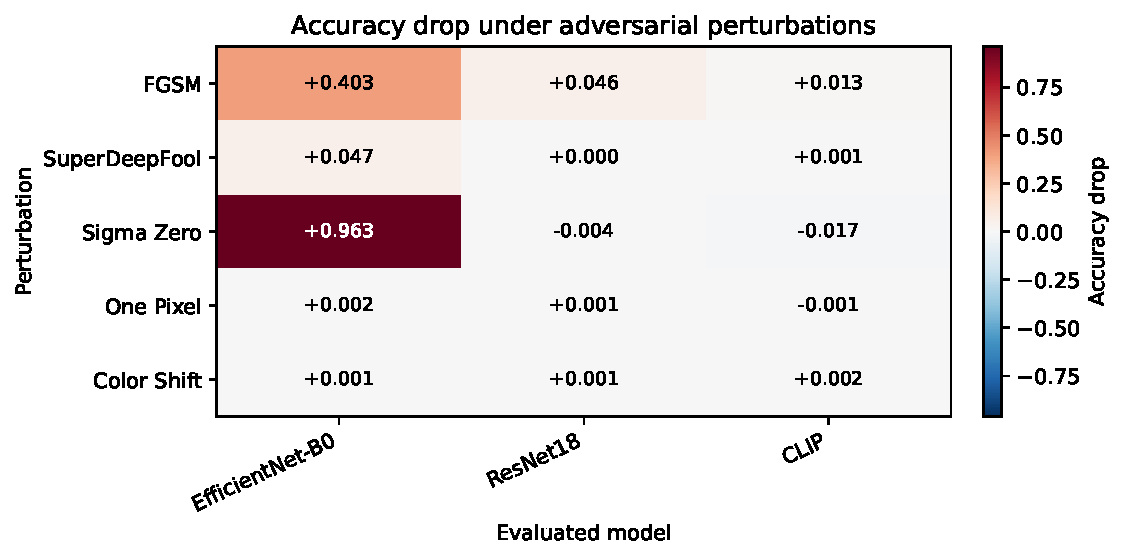
\includegraphics[width=0.88\textwidth]{images/fig_adversarial_accuracy_drop_heatmap.pdf}
\caption{Accuracy drop sotto perturbazioni adversariali. Il drop è definito come \(\text{accuracy}_{clean}-\text{accuracy}_{perturbed}\). La degradazione più marcata riguarda EfficientNet-B0 sotto \gls{sigmazero}, confermando la vulnerabilità del modello nello scenario white-box considerato.}
\label{fig:results-adversarial-accuracy-drop-heatmap}
\end{figure}

Il risultato più critico riguarda EfficientNet-B0 sotto \gls{sigmazero}, dove
l'accuracy passa da 0.978 a 0.015, con una variazione pari a -0.963. Tale valore
indica una compromissione quasi completa della capacità classificativa del
modello, limitata tuttavia alla configurazione white-box in cui l'attacco è
ottimizzato direttamente contro EfficientNet-B0 con accesso pieno ai suoi
parametri. In termini operativi, tale risultato implica un \gls{fnr} prossimo
all'unità per la classe \texttt{weapon}: nello scenario white-box considerato,
il modello diventa inadatto al triage automatico di immagini contenenti armi,
nonostante la baseline clean risulti la più elevata tra i modelli proxy.

Anche \gls{fgsm}, generato contro EfficientNet-B0, produce un degrado
rilevante, riducendo l'accuracy a 0.575 e determinando una variazione pari a
-0.403. \gls{superdeepfool} produce invece un effetto più contenuto sullo stesso
modello, con accuracy pari a 0.931 e variazione pari a -0.047.

Il confronto con ResNet18 e \gls{clip} mostra che il trasferimento degli attacchi
generati contro EfficientNet-B0 non produce una degradazione equivalente sugli
altri modelli. ResNet18 subisce una variazione pari a -0.046 sotto \gls{fgsm},
mentre rimane sostanzialmente stabile rispetto a \gls{superdeepfool},
\gls{onepixel}, \gls{sigmazero} e \gls{colorshift}. \gls{clip} mostra variazioni
ancora più contenute, con il peggioramento massimo pari a -0.013 sotto
\gls{fgsm}. In alcuni casi, come \gls{sigmazero}, l'accuracy perturbata di
\gls{clip} e ResNet18 risulta lievemente superiore alla rispettiva baseline
clean. Questo risultato suggerisce che le perturbazioni ottimizzate contro
EfficientNet-B0 alterano caratteristiche pixel-level non necessariamente
diagnostiche per ResNet18 e \gls{clip}, comportandosi per tali architetture come
una trasformazione neutra o lievemente favorevole, piuttosto che come una
perturbazione effettivamente trasferibile.

La Figura~\ref{fig:results-adversarial-accuracy-drop-heatmap} rende
visivamente evidente il contrasto tra la colonna EfficientNet-B0, dominata da
drop elevati, e le colonne ResNet18 e \gls{clip}, caratterizzate da variazioni
prossime allo zero o lievemente positive.

Dal punto di vista forense, la vulnerabilità di EfficientNet-B0 a perturbazioni
come \gls{sigmazero} e \gls{fgsm} evidenzia un rischio operativo significativo:
un sistema apparentemente molto accurato in condizioni clean può degradare in
modo drastico quando esposto a input manipolati in modo deliberato. Questo
rafforza la necessità di non interpretare l'output di un classificatore
\gls{ai}-based come evidenza autonoma, ma come supporto al triage da sottoporre
a verifica, tracciamento e validazione nel contesto complessivo dell'indagine.

% ─────────────────────────────────────────────────────────────────────────────
\section{Forensic Evaluation Bundle Composition and Black-Box Readiness}
\label{sec:results-bundle}
% ─────────────────────────────────────────────────────────────────────────────

Il forensic evaluation bundle costituisce il livello di collegamento tra la
valutazione sperimentale controllata dei modelli proxy e la successiva
valutazione black-box degli strumenti forensi commerciali. Il bundle è progettato
per fornire ai tool un input cieco e semanticamente neutro, preservando
separatamente le informazioni necessarie per il matching, la normalizzazione
degli export e l'audit dei risultati
\cite{casey2011digital,nist2006guide,iso27041,iso27042,swgde2014validation}.

A differenza della composizione generale del corpus sperimentale riportata nella
Sezione~\ref{sec:results-status}, la Tabella~\ref{tab:results-bundle-operational-layout}
descrive il bundle dal punto di vista operativo, distinguendo tra contenuto
sottoposto ai tool, naming cieco e ruolo dei metadati nella fase di audit. Il
totale è pari a 11\,500 file, comprendenti 1000 campioni clean, 500 campioni
\gls{ood}, 5000 campioni adversariali e 5000 campioni anti-forensi.

\begin{table}[H]
\centering
\scriptsize
\caption{Vista operativa del forensic evaluation bundle per la valutazione black-box.}
\label{tab:results-bundle-operational-layout}
\begin{tabularx}{\textwidth}{@{}l r l X@{}}
\toprule
\textbf{Componente} &
\textbf{File} &
\textbf{Input cieco} &
\textbf{Ruolo dei metadati} \\
\midrule
Clean &
1000 &
\texttt{bundle\_*.jpg} &
Conserva la corrispondenza con il subset binario originale e con la label
\texttt{weapon}/\texttt{non\_weapon}. \\

\gls{ood} &
500 &
\texttt{bundle\_*.jpg} &
Preserva la distinzione tra campioni fuori distribuzione e task binario
nominale. \\

Adversarial &
5000 &
\texttt{bundle\_*.jpg} &
Registra famiglia di attacco, nome della perturbazione, modello target e
immagine sorgente. \\

Anti-forensic &
5000 &
\texttt{bundle\_*.jpg} &
Registra trasformazione applicata, immagine sorgente e mapping verso il
campione clean corrispondente. \\
\midrule
\textbf{Totale} &
\textbf{11\,500} &
\texttt{bundle\_*.jpg} &
Abilita matching, normalizzazione post-export e audit hash-based. \\
\bottomrule
\end{tabularx}
\end{table}

La costruzione del bundle segue due viste complementari. La prima è una
directory cieca destinata ai tool forensi, nella quale i file sono rinominati con
identificativi neutri del tipo \texttt{bundle\_000001.jpg}. La seconda è una
vista strutturata di audit, riservata al ricercatore, nella quale sono preservate
le informazioni semantiche e sperimentali necessarie alla verifica. Per la
valutazione black-box, i tool devono importare esclusivamente la directory:

\begin{verbatim}
datasets/forensic_evaluation_bundle/blind_tool_input/files
\end{verbatim}

e non devono importare né la directory \texttt{metadata/} né la directory
\texttt{structured\_audit\_view/}. Questa separazione riduce il rischio di bias
indotto dai nomi dei file, dai path, dalle classi, dai nomi degli attacchi o
dalla struttura degli split.

Il bundle preserva la tracciabilità attraverso manifest separati contenenti, per
ciascun file, identificativo del bundle, nome cieco, tipo di campione, famiglia e
nome della perturbazione, fold, label finale, dataset sorgente, identificativo
dell'immagine originale, path sorgente, path cieco, path strutturato, hash
\gls{sha256}, hash \gls{md5}, dimensione del file ed estensione. Tale struttura
consente di collegare ogni output esportato da un tool commerciale al
corrispondente artefatto sperimentale senza esporre al tool la ground truth
durante la fase di importazione.

I controlli di consistenza confermano che gli identificativi del bundle sono
univoci, gli hash \gls{sha256} effettivi sono univoci, gli hash calcolati
corrispondono a quelli riportati nel manifest quando disponibili, i path ciechi
sono semanticamente neutri e i metadati sono separati dall'input operativo dei
tool. Questi controlli sono essenziali per rendere il bundle idoneo alla
valutazione black-box, poiché permettono di distinguere tra errori di
classificazione, file non processati, output non categorizzati, limiti del
formato di export e problemi di matching \cite{iso27041,iso27042,iso27043,swgde2014validation}.

In sintesi, il forensic evaluation bundle consente di passare da una valutazione
proxy completamente controllata a una valutazione più vicina al contesto
operativo degli strumenti forensi commerciali. La sua funzione non è soltanto
organizzativa, ma metodologica: preserva la riproducibilità dell'esperimento e
riduce l'esposizione dei tool a informazioni semantiche non necessarie. Al tempo
stesso, abilita una normalizzazione post-export basata su identificativi e hash
verificabili, condizione necessaria per distinguere errori di classificazione
genuini da artefatti del processo di export.

\section{Commercial Forensic Tools Evaluation}
\label{sec:results-commercial}

La valutazione degli strumenti forensi commerciali rappresenta il livello
black-box della pipeline sperimentale. A differenza dei modelli proxy analizzati
nelle sezioni precedenti, per i tool commerciali non sono disponibili
architettura del modello, dataset di addestramento, soglie decisionali,
preprocessing interno o logica completa di classificazione. La valutazione si
basa quindi esclusivamente sugli output osservabili prodotti dal tool, sui tag
assegnati, sulle categorie esportate e sul matching tra i file del forensic
evaluation bundle e la ground truth sperimentale.


\subsection{Black-box evaluation protocol}
\label{subsec:results-commercial-protocol}

Per evitare che il tool potesse utilizzare informazioni semantiche derivate dai
nomi dei file, dai path o dalla struttura delle cartelle, la valutazione è stata
condotta utilizzando la vista cieca del forensic evaluation bundle. I file sono
stati importati con nomi neutri del tipo \texttt{bundle\_*.jpg}, mentre le
informazioni relative a classe, sorgente, fold, attacco, trasformazione, hash e
ground truth sono state mantenute separate nei manifest di audit.

Dopo l'elaborazione da parte del tool, gli output esportati sono stati
normalizzati e ricondotti ai campioni originali tramite identificativi del
bundle e hash crittografici. Questa impostazione consente di distinguere tra
immagini correttamente segnalate, immagini non segnalate, falsi negativi sulla
classe \texttt{weapon}, falsi positivi sulle classi \texttt{non\_weapon} e
\gls{ood}, e differenze di comportamento tra input clean, adversariali e
anti-forensi.



\subsection{Tool availability and export normalization}
\label{subsec:results-commercial-availability}

La Tabella~\ref{tab:results-commercial-tool-status} riassume lo stato della
valutazione dei tool commerciali considerati. In questa versione dei risultati,
la valutazione quantitativa black-box è consolidata per Magnet AXIOM/Magnet.AI
e per X-Ways Forensics/Excire Photo AI. I due strumenti non sono tuttavia
equivalenti dal punto di vista funzionale: Magnet.AI espone un tag operativo
riconducibile alla categoria \texttt{Possible weapons}, mentre Excire Photo AI è
stato valutato come sistema di ricerca semantica visuale, nel quale la decisione
operativa dipende dal recupero o meno dell'immagine rispetto a query e soglie di
similarità configurate.

Per tale ragione, Excire non viene trattato come classificatore nativo
\texttt{weapon}/\texttt{non\_weapon}, ma come semantic retrieval-based
classifier. La sensitivity analysis sul parametro \texttt{Distance limit}
consente di osservare come il comportamento operativo cambi al variare della
soglia: \texttt{D20} rappresenta una configurazione restrittiva, \texttt{D50}
una configurazione intermedia orientata al triage forense, e \texttt{D80} una
configurazione permissiva ad alto richiamo.

\begin{table}[H]
\centering
\scriptsize
\renewcommand{\arraystretch}{1.15}
\setlength{\tabcolsep}{4pt}
\caption{Stato della valutazione black-box degli strumenti forensi commerciali.}
\label{tab:results-commercial-tool-status}
\begin{tabularx}{\textwidth}{@{}p{0.26\textwidth} p{0.20\textwidth} X@{}}
\toprule
\textbf{Tool / configurazione} & \textbf{Stato} & \textbf{Implicazione metodologica} \\
\midrule

Magnet.AI &
Consolidato &
Export normalizzato rispetto alla ground truth; il tag \texttt{Possible weapons} è usato come segnale operativo positivo per \texttt{weapon}. \\

Excire \texttt{D20} &
Consolidato &
Configurazione restrittiva: riduce falsi positivi e segnalazioni \gls{ood}, ma aumenta il rischio di falsi negativi. \\

Excire \texttt{D50} &
Consolidato &
Configurazione intermedia adottata come riferimento principale per il confronto operativo. \\

Excire \texttt{D80} &
Consolidato &
Configurazione permissiva: massimizza il recall, ma aumenta \gls{fpr} e weapon flag rate sugli input \gls{ood}. \\

Cellebrite UFED &
Fuori confronto quantitativo &
Rilevante nel workflow forense, ma non valutato quantitativamente per assenza di export normalizzati comparabili. \\

Oxygen Forensic Detective &
Fuori confronto quantitativo &
Non incluso nella comparazione quantitativa finale per assenza di output strutturati e mappabili alla ground truth. \\

\bottomrule
\end{tabularx}
\end{table}

La Figura~\ref{fig:results-forensic-tools-clean-comparison} visualizza il
confronto delle metriche clean tra Magnet.AI ed Excire Photo AI, evidenziando il
diverso bilanciamento tra recall, falsi negativi e falsi positivi nelle tre
configurazioni di Excire.

\begin{figure}[H]
\centering

\includegraphics[width=0.88\textwidth]{images/fig_forensic_tools_clean_metrics_comparison.pdf}
\caption{Confronto delle metriche clean per Magnet.AI ed Excire Photo AI nelle configurazioni \texttt{D20}, \texttt{D50} e \texttt{D80}.}
\label{fig:results-forensic-tools-clean-comparison}
\end{figure}



Per Magnet AXIOM/Magnet.AI, la normalizzazione è stata condotta sul run
\texttt{FAIRLAB\_AXIOM\_RUN\_02}, selezionato come esportazione di riferimento
per la completezza e la consistenza degli output prodotti. Nel run selezionato
sono stati individuati cinque file di export complessivi, di cui un file
predittivo principale utilizzato per ricostruire le segnalazioni
\texttt{Possible weapons}.

Per X-Ways Forensics/Excire Photo AI, la normalizzazione è stata condotta su tre
run distinti, corrispondenti alle configurazioni \texttt{D20}, \texttt{D50} e
\texttt{D80}. Le tre configurazioni non rappresentano ripetizioni dello stesso
esperimento e non devono quindi essere mediate tra loro: ciascuna descrive un
profilo operativo differente del sistema di semantic retrieval.

\subsection{Magnet AXIOM / Magnet.AI results}
\label{subsec:results-magnet}

La valutazione di Magnet AXIOM/Magnet.AI costituisce il primo risultato
black-box commerciale consolidato della pipeline. Gli output prodotti dal tool
sono stati normalizzati mappando il tag \texttt{Possible weapons} come
predizione positiva per la classe \texttt{weapon} e l'assenza di tag come
predizione negativa. La normalizzazione ha prodotto un match completo tra export
del tool e forensic evaluation bundle: tutte le 11\,500 immagini sono state
ricondotte a un identificativo del bundle e nessuna riga è rimasta unmatched.

Questa normalizzazione deve essere interpretata come una ricodifica operativa
dell'output esportato dal tool, non come accesso alla decisione interna del
modulo proprietario. Di conseguenza, le metriche riportate descrivono il
comportamento osservabile del sistema rispetto al bundle sperimentale, non le
prestazioni intrinseche del modello interno eventualmente utilizzato dal tool.


\begin{table}[H]
\centering
\caption{Sintesi della normalizzazione dell'export Magnet AXIOM/Magnet.AI.}
\label{tab:results-magnet-normalization-summary}
\small
\begin{tabular}{lr}
\toprule
\textbf{Elemento} & \textbf{Valore} \\
\midrule
Immagini nel forensic evaluation bundle & 11\,500 \\
Righe normalizzate dopo deduplicazione & 11\,500 \\
Righe matched & 11\,500 \\
Righe unmatched & 0 \\
Predizioni interpretabili & 11\,500 \\
Predizioni \texttt{weapon\_detected=true} & 5\,329 \\
Predizioni \texttt{weapon\_detected=false} & 6\,171 \\
Predizioni \texttt{weapon\_detected=unknown} & 0 \\
\bottomrule
\end{tabular}
\end{table}

Sulle sole classi binarie \texttt{weapon} e \texttt{non\_weapon}, escludendo le
500 immagini \gls{ood}, Magnet.AI raggiunge un'accuracy complessiva pari a
0.933 e una precisione sulla classe \texttt{weapon} pari a 0.963. Tuttavia, il
recall sulla classe \texttt{weapon} è pari a 0.901, con un \gls{fnr} di 0.099:
542 immagini appartenenti alla classe \texttt{weapon} non sono state segnalate
come \texttt{Possible weapons}.

\begin{table}[H]
\centering
\caption{Prestazioni complessive di Magnet.AI sul task binario weapon/non\_weapon.}
\label{tab:results-magnet-global-metrics}
\small
\begin{tabular}{lr}
\toprule
\textbf{Metrica} & \textbf{Valore} \\
\midrule
Accuracy & 0.933 \\
Precision \texttt{weapon} & 0.963 \\
Recall \texttt{weapon} & 0.901 \\
F1 \texttt{weapon} & 0.931 \\
False negative rate & 0.099 \\
False positive rate & 0.035 \\
True positives & 4\,958 \\
True negatives & 5\,309 \\
False positives & 191 \\
False negatives & 542 \\
\bottomrule
\end{tabular}
\end{table}

Le metriche complessive riportate nella Tabella~\ref{tab:results-magnet-global-metrics}
sono calcolate sulle 11\,000 immagini appartenenti al task binario
\texttt{weapon}/\texttt{non\_weapon}. Il valore globale non corrisponde alla
media aritmetica semplice tra clean e perturbed, poiché il bundle contiene
1\,000 immagini clean e 10\,000 immagini perturbate. Di conseguenza, le
condizioni perturbate hanno peso maggiore nella metrica aggregata.

\begin{table}[H]
\centering
\caption{Comportamento di Magnet.AI per condizione sperimentale.}
\label{tab:results-magnet-condition-metrics}
\small
\begin{tabularx}{\textwidth}{@{}l r r r r X@{}}
\toprule
\textbf{Condizione} &
\textbf{Accuracy} &
\textbf{Recall weapon} &
\textbf{\gls{fnr}} &
\textbf{\gls{fpr}} &
\textbf{Nota operativa} \\
\midrule

Clean &
0.950 &
0.930 &
0.070 &
0.030 &
Baseline commerciale su 1\,000 immagini non perturbate. \\

Perturbed &
0.932 &
0.899 &
0.101 &
0.035 &
Valori calcolati su 10\,000 immagini adversariali e anti-forensi; il degrado
principale riguarda l'aumento dei falsi negativi sulla classe \texttt{weapon}. \\

OOD &
-- &
-- &
-- &
-- &
Weapon flag rate pari a 0.360: 180 immagini \gls{ood} su 500 sono state
segnalate come \texttt{Possible weapons}. Le metriche binarie standard non sono
applicabili. \\

\bottomrule
\end{tabularx}
\end{table}

Tra le condizioni perturbate, gli attacchi adversariali producono una
degradazione più marcata rispetto alle trasformazioni anti-forensi: il
\gls{fnr} medio adversariale è pari a 0.116, contro 0.087 per le trasformazioni
anti-forensi. Questo risultato conferma che, nel caso di Magnet.AI, le
perturbazioni progettate per interferire con il comportamento del classificatore
hanno un impatto operativo superiore rispetto alle trasformazioni realistiche di
degradazione o manipolazione dell'immagine.

Il risultato sulle immagini \gls{ood} è particolarmente rilevante per il
workflow di triage. Le immagini fuori distribuzione non appartengono al task
binario weapon/non\_weapon e non devono quindi essere interpretate come errori
classici di classificazione. Tuttavia, il fatto che 180 immagini \gls{ood} su
500 siano state segnalate come \texttt{Possible weapons} indica che il modulo
automatico può assegnare rilevanza investigativa a contenuti semanticamente
ambigui o non appartenenti alla distribuzione attesa.

A differenza dei modelli proxy, Magnet.AI non esporta valori di confidenza
numerici associati alle singole predizioni. La classificazione osservabile si
basa esclusivamente sulla presenza o assenza del tag \texttt{Possible weapons},
senza indicazione quantitativa del grado di certezza. Questa caratteristica
preclude il confronto diretto con le distribuzioni di confidenza dei modelli
proxy e costituisce un ulteriore limite alla tracciabilità dell'output.

La Tabella~\ref{tab:results-magnet-attack-metrics} riporta le condizioni più
rilevanti tra attacchi adversariali e trasformazioni anti-forensi. FGSM risulta
la condizione più critica per Magnet.AI, con accuracy pari a 0.867, recall
\texttt{weapon} pari a 0.808 e \gls{fnr} pari a 0.192.

\begin{table}[H]
\centering
\caption{Prestazioni di Magnet.AI nelle principali condizioni perturbate.}
\label{tab:results-magnet-attack-metrics}
\small
\begin{tabular}{l r r r r r r}
\toprule
\textbf{Condizione} &
\textbf{Accuracy} &
\textbf{Recall} &
\textbf{\gls{fnr}} &
\textbf{\gls{fpr}} &
\textbf{FN} &
\textbf{FP} \\
\midrule

FGSM &
0.867 &
0.808 &
0.192 &
0.074 &
96 &
37 \\

Sigma Zero &
0.916 &
0.856 &
0.144 &
0.024 &
72 &
12 \\

SuperDeepFool &
0.932 &
0.894 &
0.106 &
0.030 &
53 &
15 \\

Gaussian Blur &
0.927 &
0.880 &
0.120 &
0.026 &
60 &
13 \\

Histogram Modification &
0.936 &
0.920 &
0.080 &
0.048 &
40 &
24 \\

\bottomrule
\end{tabular}
\end{table}

Nel complesso, Magnet.AI mostra prestazioni elevate in condizioni clean, ma
evidenzia una riduzione della capacità di segnalazione della classe
\texttt{weapon} in presenza di perturbazioni adversariali. Il dato più rilevante
non è la sola riduzione di accuracy, ma l'aumento dei falsi negativi: in uno
scenario di triage, un'immagine \texttt{weapon} non segnalata dal modulo
automatico può ricevere minore priorità di revisione umana.

Questi risultati devono essere interpretati come indicatori di affidabilità
operativa, non come misura della robustezza algoritmica interna di Magnet.AI,
che rimane non ispezionabile. Il tool mantiene buone prestazioni complessive e
una precisione elevata sulla classe \texttt{weapon}, ma produce falsi negativi
in condizioni clean e perturbate e segnala una quota non trascurabile di immagini
\gls{ood} come \texttt{Possible weapons}. Questi risultati confermano che
l'output automatico deve essere trattato come supporto al triage e non come
decisione conclusiva o autosufficiente.



\subsection{X-Ways / Excire Photo AI results and sensitivity analysis}
\label{subsec:results-excire}

La valutazione di X-Ways Forensics/Excire Photo AI richiede una cautela
interpretativa specifica. A differenza di Magnet.AI, Excire non è stato trattato
come un classificatore nativo per la distinzione binaria
\texttt{weapon}/\texttt{non\_weapon}, ma come un sistema black-box di semantic
retrieval. La predizione operativa è stata quindi derivata dalla presenza o
assenza del campione tra i risultati recuperati dal tool rispetto alla ricerca
semantica configurata. Questa ricodifica consente una valutazione quantitativa
rispetto alla ground truth sperimentale, ma non deve essere interpretata come
accesso alla logica classificatoria interna del sistema.

Per valutare la sensibilità del comportamento operativo alla soglia di recupero,
sono state considerate tre configurazioni del parametro \texttt{Distance limit}.
La configurazione \texttt{D20} rappresenta un'impostazione restrittiva, orientata
a ridurre falsi positivi e recuperi semanticamente deboli. \texttt{D50} rappresenta, nel contesto sperimentale considerato, una
configurazione intermedia orientata al triage, poiché mantiene un recall elevato
sulla classe \texttt{weapon} senza produrre il livello di rumore osservato in
\texttt{D80}. La configurazione \texttt{D80} rappresenta invece un'impostazione permissiva,
orientata a massimizzare il recall ma esposta a un aumento rilevante dei falsi
positivi.

\begin{table}[H]
\centering
\scriptsize
\renewcommand{\arraystretch}{1.15}
\setlength{\tabcolsep}{4pt}
\caption{Sensitivity analysis di Excire Photo AI rispetto al parametro \texttt{Distance limit}.}
\label{tab:results-excire-sensitivity}
\begin{tabularx}{0.95\textwidth}{@{}l r r r r r X@{}}
\toprule
\textbf{Setting} &
\textbf{Acc.} &
\textbf{Recall} &
\textbf{\gls{fnr}} &
\textbf{\gls{fpr}} &
\textbf{OOD rate} &
\textbf{Profilo operativo} \\
\midrule

\texttt{D20} &
0.927 &
0.880 &
0.120 &
0.026 &
0.238 &
Restrittivo: basso rumore, maggiore rischio di falsi negativi. \\

\texttt{D50} &
0.944 &
0.958 &
0.042 &
0.070 &
0.340 &
Intermedio: compromesso equilibrato nel contesto sperimentale. \\

\texttt{D80} &
0.915 &
0.986 &
0.014 &
0.156 &
0.522 &
Permissivo: alto recall, maggiore rumore operativo. \\

\bottomrule
\end{tabularx}
\end{table}

Il confronto tra le tre configurazioni conferma che il parametro
\texttt{Distance limit} non agisce come una semplice variabile tecnica, ma come
una soglia operativa che modifica il profilo di rischio del tool. \texttt{D20}
è più conservativo e riduce il carico di revisione derivante da falsi positivi,
ma può non recuperare contenuti \texttt{weapon} rilevanti. \texttt{D50} rappresenta, nel contesto sperimentale considerato, una
configurazione intermedia orientata al triage, poiché mantiene un recall elevato
sulla classe \texttt{weapon} senza produrre il livello di rumore osservato in
\texttt{D80}. Quest'ultimo, pur riducendo drasticamente i
falsi negativi, incrementa in modo sostanziale i falsi positivi e segnala come
rilevante oltre la metà degli input \gls{ood}.



La Figura~\ref{fig:results-forensic-tools-ood-weapon-flag-rate} mostra
visivamente come il weapon flag rate sugli input \gls{ood} vari al variare della
configurazione operativa, confermando che il parametro \texttt{Distance limit}
incide direttamente sul profilo di rischio del sistema.


\begin{figure}[H]
\centering
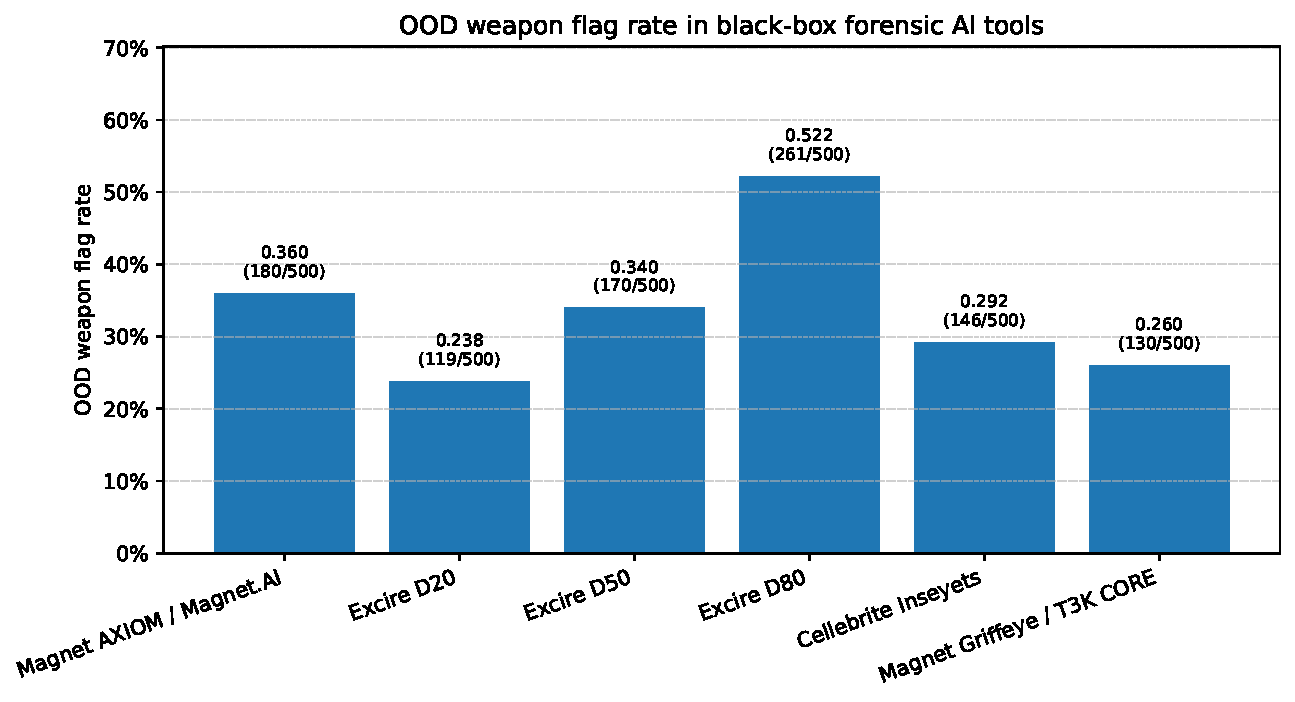
\includegraphics[width=0.82\textwidth]{images/fig_forensic_tools_ood_weapon_flag_rate.pdf}
\caption{Weapon flag rate sugli input \gls{ood} per Magnet.AI ed Excire Photo AI nelle configurazioni \texttt{D20}, \texttt{D50} e \texttt{D80}.}
\label{fig:results-forensic-tools-ood-weapon-flag-rate}
\end{figure}



\begin{table}[H]
\centering
\caption{Prestazioni aggregate di Excire Photo AI sulle condizioni perturbate.}
\label{tab:results-excire-perturbed-summary}
\small
\begin{tabular}{l l r r r r}
\toprule
\textbf{Setting} &
\textbf{Condizione} &
\textbf{Accuracy} &
\textbf{Recall weapon} &
\textbf{\gls{fnr}} &
\textbf{\gls{fpr}} \\
\midrule

\texttt{D20} & Anti-forensic & 0.927 & 0.875 & 0.125 & 0.022 \\
\texttt{D50} & Anti-forensic & 0.941 & 0.957 & 0.043 & 0.074 \\
\texttt{D80} & Anti-forensic & 0.908 & 0.984 & 0.016 & 0.169 \\
\midrule
\texttt{D20} & Adversarial & 0.892 & 0.834 & 0.166 & 0.051 \\
\texttt{D50} & Adversarial & 0.904 & 0.938 & 0.062 & 0.130 \\
\texttt{D80} & Adversarial & 0.861 & 0.977 & 0.023 & 0.256 \\

\bottomrule
\end{tabular}
\end{table}

I risultati aggregati sulle condizioni perturbate confermano che le
trasformazioni anti-forensi producono un impatto contenuto rispetto agli attacchi
adversariali. Anche in questo caso, tuttavia, il profilo operativo cambia in modo
sostanziale al variare della soglia: \texttt{D20} mantiene il \gls{fpr} più
basso ma presenta il \gls{fnr} più elevato, \texttt{D80} riduce quasi
completamente i falsi negativi ma incrementa il rumore operativo, mentre
\texttt{D50} mantiene un compromesso intermedio tra richiamo e selettività nel
contesto sperimentale considerato.

La Figura~\ref{fig:results-forensic-tools-attack-family-fpr} sintetizza il
\gls{fpr} aggregato per famiglia di perturbazione, rendendo più evidente il
diverso contributo delle condizioni adversariali e anti-forensi al rumore
operativo prodotto dai tool commerciali.


\begin{figure}[H]
\centering
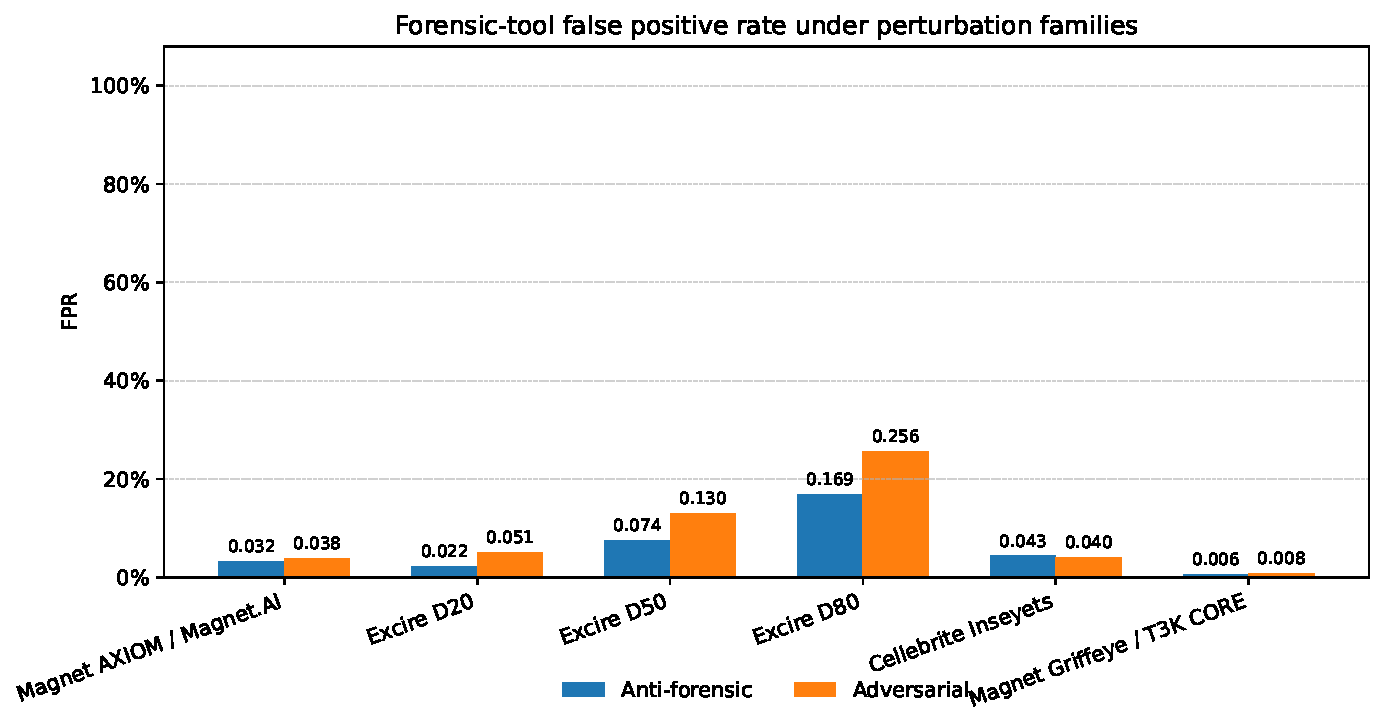
\includegraphics[width=0.84\textwidth]{images/fig_forensic_tools_attack_family_fpr.pdf}
\caption{\gls{fpr} aggregato dei tool commerciali per famiglia di perturbazione.}
\label{fig:results-forensic-tools-attack-family-fpr}
\end{figure}



Un caso particolarmente rilevante è rappresentato da \gls{sigmazero}. A
differenza di una semplice dinamica di evasione, in cui l'effetto principale
sarebbe l'aumento dei falsi negativi sulla classe \texttt{weapon}, Excire mostra
nelle configurazioni \texttt{D50} e \texttt{D80} un comportamento di
over-triggering semantico. In tali condizioni, il sistema continua a recuperare
molte immagini \texttt{weapon}, ma aumenta in modo molto marcato la quota di
immagini \texttt{non\_weapon} erroneamente recuperate come rilevanti.

\begin{table}[H]
\centering
\caption{Comportamento dei tool commerciali sulla perturbazione \gls{sigmazero}.}
\label{tab:results-commercial-sigma-zero}
\small
\begin{tabular}{l r r r r r r}
\toprule
\textbf{Tool / setting} &
\textbf{Accuracy} &
\textbf{Recall} &
\textbf{\gls{fnr}} &
\textbf{\gls{fpr}} &
\textbf{FN} &
\textbf{FP} \\
\midrule

Magnet.AI & 0.916 & 0.856 & 0.144 & 0.024 & 72 & 12 \\
Excire \texttt{D20} & 0.815 & 0.820 & 0.180 & 0.190 & 90 & 95 \\
Excire \texttt{D50} & 0.742 & 0.926 & 0.074 & 0.442 & 37 & 221 \\
Excire \texttt{D80} & 0.657 & 0.976 & 0.024 & 0.662 & 12 & 331 \\

\bottomrule
\end{tabular}
\end{table}

La Figura~\ref{fig:results-forensic-tools-adversarial-drop} riporta l'accuracy
drop dei tool commerciali sotto perturbazioni adversariali, fornendo un supporto
visivo alla lettura del comportamento anomalo osservato su \gls{sigmazero}.

\begin{figure}[H]
\centering

\includegraphics[width=0.88\textwidth]{images/fig_forensic_tools_adversarial_accuracy_drop_heatmap.pdf}
\caption{Accuracy drop dei tool commerciali black-box sotto perturbazioni adversariali.}
\label{fig:results-forensic-tools-adversarial-drop}
\end{figure}


Questo comportamento è operativo-forensicamente significativo. In un workflow di
triage, una configurazione permissiva può sembrare preferibile perché riduce il
rischio di mancata segnalazione, ma può generare un volume elevato di falsi
positivi, saturando la revisione umana e riducendo l'efficienza del filtro
automatico. Pertanto, nel caso di Excire, \gls{sigmazero} non evidenzia soltanto
una vulnerabilità di evasione, ma anche un rischio di amplificazione del rumore
semantico.



\subsection{Commercial tools not included in the quantitative comparison}
\label{subsec:results-commercial-not-included}

Cellebrite UFED e Oxygen Forensic Detective rimangono rilevanti nel workflow
operativo-forense della tesi, ma non sono inclusi nella comparazione quantitativa
finale del Capitolo~\ref{chap:results}. La ragione non riguarda la loro
irrilevanza investigativa, bensì la mancanza, nella presente fase sperimentale,
di output normalizzati, riproducibili e comparabili rispetto al forensic
evaluation bundle.

In particolare, l'inclusione quantitativa di un tool commerciale richiede che i
risultati esportati siano associabili in modo univoco ai file del bundle, tramite
nome normalizzato, path, identificativo interno o hash, e che il significato
operativo della categoria esportata possa essere ricondotto in modo documentato
alla ground truth sperimentale. In assenza di tali condizioni, l'inserimento del
tool in una tabella comparativa rischierebbe di introdurre una falsa equivalenza
metodologica tra sistemi con output non omogenei.

Pertanto, la valutazione quantitativa commerciale è consolidata per Magnet
AXIOM/Magnet.AI e per X-Ways Forensics/Excire Photo AI, mentre UFED e Oxygen
sono mantenuti come strumenti della pipeline operativo-forense da discutere sul
piano metodologico e procedurale.



\section{Comparative Robustness Discussion}
\label{sec:results-comparative}

I risultati ottenuti consentono di confrontare tre livelli della pipeline:
modelli proxy trasparenti, perturbazioni sperimentali controllate e valutazione
black-box commerciale. I modelli proxy permettono di osservare in modo
controllato il degrado prestazionale rispetto a clean, \gls{ood}, adversarial e
anti-forensic input. Magnet.AI ed Excire Photo AI permettono invece di verificare
come strumenti professionali black-box reagiscano allo stesso bundle
sperimentale, pur senza accesso alla logica interna del classificatore o del
motore di retrieval.

La Tabella~\ref{tab:results-comparative-summary} sintetizza i principali
risultati comparativi. Il confronto non deve essere interpretato come ranking
diretto tra modelli proxy e tool commerciali, perché i primi espongono
predizioni controllate su classi binarie note, mentre i secondi operano tramite
categorie proprietarie, tag esportati o recupero semantico. Il valore del
confronto è operativo: mostrare se le tendenze di fragilità osservate nei proxy
si riflettono anche in strumenti black-box utilizzati in workflow investigativi.

\begin{table}[H]
\centering
\caption{Sintesi comparativa tra modelli proxy e tool commerciali black-box.}
\label{tab:results-comparative-summary}
\small
\begin{tabularx}{\textwidth}{@{}p{2.4cm} r r r X@{}}
\toprule
\textbf{Sistema} &
\textbf{Clean accuracy} &
\textbf{Clean \gls{fnr}} &
\textbf{OOD weapon rate} &
\textbf{Osservazione principale} \\
\midrule

EfficientNet-B0 &
0.978 &
0.016 &
0.370 &
Migliore baseline clean tra i proxy, ma vulnerabilità marcata ad alcune
perturbazioni adversariali, in particolare \gls{sigmazero} e \gls{fgsm}. \\

ResNet18 &
0.964 &
0.030 &
0.438 &
Buona baseline e maggiore stabilità rispetto a EfficientNet-B0 in alcuni
scenari adversariali, pur con vulnerabilità osservabili. \\

\gls{clip} &
0.927 &
0.012 &
0.836 &
Accuracy clean inferiore ai modelli supervisionati, ma forte tendenza a
segnalare come \texttt{weapon} immagini fuori distribuzione. \\

Magnet AXIOM / Magnet.AI &
0.950 &
0.070 &
0.360 &
Comportamento relativamente conservativo: basso \gls{fpr}, ma rischio non
trascurabile di falsi negativi sulla classe \texttt{weapon}. \\

X-Ways / Excire Photo AI \texttt{D50} &
0.944 &
0.042 &
0.340 &
Setting principale di triage: recall elevato sulla classe \texttt{weapon}, con
incremento controllato dei falsi positivi rispetto alle configurazioni più
permissive. \\

\bottomrule
\end{tabularx}
\end{table}

Excire \texttt{D20} e \texttt{D80} non sono inclusi nella tabella come valori da
mediare con \texttt{D50}, poiché rappresentano configurazioni operative diverse.
\texttt{D20} descrive un uso restrittivo del semantic retrieval, adatto a
contenere falsi positivi e segnalazioni \gls{ood}; \texttt{D80} descrive invece
un uso permissivo, utile quando l'obiettivo prioritario è massimizzare il recall,
ma con un aumento rilevante del rumore operativo. La configurazione
\texttt{D50} viene quindi adottata come riferimento principale per il confronto
con Magnet.AI, mentre \texttt{D20} e \texttt{D80} sono interpretate come
sensitivity analysis.

Una divergenza rilevante emerge nel confronto tra \gls{clip}, i modelli
supervisionati e i tool commerciali. \gls{clip} mostra un weapon rate su
immagini \gls{ood} molto più alto rispetto a EfficientNet-B0 e ResNet18, pur con
una confidenza media inferiore. Magnet.AI ed Excire \texttt{D50} mostrano invece
weapon flag rate più contenuti, rispettivamente pari a 0.360 e 0.340. Questo non
rende automaticamente tali strumenti più affidabili in senso assoluto, ma indica
che il comportamento su input fuori distribuzione dipende sia dall'architettura
del sistema sia dalla configurazione operativa adottata.

Questa differenza conferma che la robustezza non può essere dedotta dalla sola
accuracy clean, ma deve essere valutata rispetto a condizioni specifiche di
impiego, inclusi input anomali, borderline o semanticamente distanti dalla
distribuzione attesa. Nei workflow di \gls{df}, il problema non è soltanto
stabilire quale sistema sia più accurato in condizioni nominali, ma comprendere
quale profilo di errore esso introduca nel processo di triage: mancata
segnalazione di contenuti rilevanti, aumento del rumore operativo, assorbimento
di casi \gls{ood} o sensibilità a perturbazioni mirate.


\section{Explainability Analysis and Representative Failure Cases}
\label{sec:results-xai}

L'analisi di \gls{xai} è stata utilizzata come strumento qualitativo e
diagnostico per collegare le metriche aggregate discusse nelle sezioni
precedenti a un insieme ristretto di casi rappresentativi. Essa non costituisce
una metrica primaria di robustezza e non sostituisce le misure quantitative di
accuracy, confidence, falsi positivi e falsi negativi. Il suo ruolo è invece
quello di supportare l'interpretazione operativa di alcuni comportamenti
osservati nel modello proxy, evidenziando quali regioni dell'immagine abbiano
contribuito alla decisione del classificatore in specifici scenari di successo
o fallimento.

Le mappe di attribuzione sono state generate mediante \gls{ig} sul modello
proxy white-box EfficientNet-B0, utilizzando come target di attribuzione la
classe predetta dal modello, indicata nei file sperimentali come
\texttt{predicted\_label}. Questa scelta consente di analizzare non ciò che il
modello avrebbe dovuto riconoscere secondo l'etichetta manuale, ma ciò che ha
effettivamente guidato la decisione prodotta. Di conseguenza, nei casi errati,
la visualizzazione è orientata a comprendere quali elementi visivi abbiano
sostenuto la classificazione sbagliata.

Le mappe prodotte non devono essere interpretate come spiegazioni dirette del
comportamento di \gls{axiom}/\gls{magnetai}, \gls{xways}/\gls{excire},
\gls{ufed} o \gls{oxygen}, che rimangono strumenti commerciali black-box. Esse
forniscono invece un riferimento diagnostico controllato, limitato al modello
proxy white-box, utile per discutere in modo più concreto alcuni rischi
operativi osservabili in un contesto \gls{df} human-in-the-loop.

La Tabella~\ref{tab:results-xai-cases} riassume i cinque casi selezionati per
l'analisi qualitativa. La selezione copre un caso corretto su input pulito, un
falso negativo su input pulito, un caso \gls{ood} classificato come
\texttt{weapon}, un falso negativo prodotto da una trasformazione anti-forense
e un falso positivo adversarial ad alta confidenza.

\begin{table}[htbp]
\centering
\small
\renewcommand{\arraystretch}{1.15}
\begin{tabular}{p{0.18\textwidth} p{0.18\textwidth} p{0.15\textwidth} p{0.15\textwidth} p{0.22\textwidth}}
\toprule
\textbf{Identificativo} &
\textbf{Scenario} &
\textbf{Etichetta manuale} &
\textbf{Predizione} &
\textbf{Ruolo operativo} \\
\midrule
\texttt{xai\_case\_0001} &
\texttt{clean} &
\texttt{weapon} &
\texttt{weapon} &
Caso corretto su input pulito, utilizzato come riferimento per osservare un comportamento attributivo coerente. \\
\texttt{xai\_case\_0006} &
\texttt{clean} &
\texttt{weapon} &
\texttt{non\_weapon} &
Falso negativo su input pulito, rappresentativo di una mancata rilevazione in assenza di perturbazioni. \\
\texttt{xai\_case\_0009} &
\texttt{ood} &
\texttt{ood} &
\texttt{weapon} &
Campione \gls{ood} classificato come \texttt{weapon}, rappresentativo del rischio di inclusione semantica impropria. \\
\texttt{xai\_case\_0010} &
\texttt{histogram modification} &
\texttt{weapon} &
\texttt{non\_weapon} &
Falso negativo anti-forense, rappresentativo degli effetti di manipolazioni visuali a basso livello. \\
\texttt{xai\_case\_0015} &
\texttt{sigma\_zero} &
\texttt{non\_weapon} &
\texttt{weapon} &
Falso positivo adversarial ad alta confidenza, rappresentativo dell'inaffidabilità della sola confidence in presenza di attacco. \\
\bottomrule
\end{tabular}
\caption{Casi rappresentativi selezionati per l'analisi qualitativa di EfficientNet-B0 mediante \gls{ig}.}
\label{tab:results-xai-cases}
\end{table}

\providecommand{\XAIcaseFigure}[9]{%
\begin{figure}[htbp]
\centering
\begin{minipage}{0.44\textwidth}
\centering
\includegraphics[width=\linewidth]{#3}
\vspace{0.5mm}

{\footnotesize Immagine di input}
\end{minipage}
\hfill
\begin{minipage}{0.44\textwidth}
\centering
\includegraphics[width=\linewidth]{#4}
\vspace{0.5mm}

{\footnotesize Heatmap \gls{ig}}
\end{minipage}

\vspace{2mm}

{\small
\textit{scenario}: \texttt{#6}
\quad
$\rightarrow$
\quad
\textit{predizione}: \texttt{#8}
\quad
(\textit{etichetta manuale}: \texttt{#7}; \textit{confidenza}: #9)
}

\vspace{2mm}

\begin{minipage}{0.62\textwidth}
\centering
\includegraphics[width=\linewidth]{#5}
\vspace{0.5mm}

{\footnotesize Overlay basato su \gls{ig}}
\end{minipage}

\caption{#2}
\label{#1}
\end{figure}
}

\XAIcaseFigure
{fig:xai-case1-clean-correct}
{Caso corretto su input pulito \texttt{xai\_case\_0001}. Il modello proxy EfficientNet-B0 classifica correttamente un'immagine \texttt{clean} con etichetta manuale \texttt{weapon} come \texttt{weapon}.}
{images/fig_xai_case1_clean_correct_input.png}
{images/fig_xai_case1_clean_correct_heatmap.png}
{images/fig_xai_case1_clean_correct_overlay.png}
{clean}
{weapon}
{weapon}
{0.9999998808}

Il primo caso, mostrato in Figura~\ref{fig:xai-case1-clean-correct}, fornisce
un riferimento qualitativo in cui la predizione del modello è coerente con
l'etichetta manuale. L'immagine appartiene allo scenario \texttt{clean}, la
classe attesa è \texttt{weapon} e la predizione prodotta da EfficientNet-B0 è
anch'essa \texttt{weapon}, con confidenza molto elevata. In questo caso, la
mappa \gls{ig} è utile per verificare se il pattern attributivo sia
compatibile con la regione visivamente rilevante dell'immagine, anziché essere
dominato da elementi marginali, sfondo o artefatti di acquisizione. Tale esempio
non dimostra, da solo, l'affidabilità generale del modello, ma costituisce un
caso di riferimento rispetto al quale confrontare i fallimenti successivi.

\XAIcaseFigure
{fig:xai-case2-clean-false-negative}
{Falso negativo su input pulito \texttt{xai\_case\_0006}. Un'immagine \texttt{clean} con etichetta manuale \texttt{weapon} viene classificata come \texttt{non\_weapon}.}
{images/fig_xai_case2_clean_false_negative_input.png}
{images/fig_xai_case2_clean_false_negative_heatmap.png}
{images/fig_xai_case2_clean_false_negative_overlay.png}
{clean}
{weapon}
{non\_weapon}
{0.6920745373}

Il secondo caso, riportato in Figura~\ref{fig:xai-case2-clean-false-negative},
è rilevante perché l'errore avviene su un input pulito, senza perturbazioni
adversariali o trasformazioni anti-forensi. L'immagine è etichettata
manualmente come \texttt{weapon}, ma EfficientNet-B0 la classifica come
\texttt{non\_weapon} con confidenza moderata. In un workflow di \gls{df}, un
errore di questo tipo può produrre un rischio operativo concreto, poiché un falso
negativo può impedire che un'immagine potenzialmente rilevante venga
prioritizzata nella fase di triage automatizzato.

La corrispondente mappa \gls{ig} consente di osservare se la decisione del
modello sia sostenuta da regioni effettivamente pertinenti oppure se
l'attribuzione appaia dispersa, parziale o influenzata da elementi contestuali.
Questo caso conferma che anche una buona performance aggregata su dati
\texttt{clean} non elimina la necessità di una validazione umana, soprattutto
quando il risultato automatico viene utilizzato per filtrare o ordinare grandi
volumi di immagini in un contesto investigativo.

\XAIcaseFigure
{fig:xai-case3-ood-as-weapon}
{Caso \gls{ood} \texttt{xai\_case\_0009}. Un campione fuori distribuzione viene classificato come \texttt{weapon} con elevata confidenza.}
{images/fig_xai_case3_ood_as_weapon_input.png}
{images/fig_xai_case3_ood_as_weapon_heatmap.png}
{images/fig_xai_case3_ood_as_weapon_overlay.png}
{ood}
{ood}
{weapon}
{0.9990302324}

Il terzo caso, mostrato in Figura~\ref{fig:xai-case3-ood-as-weapon}, illustra
un rischio differente rispetto al falso positivo ordinario. Il campione è
etichettato come \texttt{ood}, ma viene assorbito dalla frontiera decisionale
binaria e classificato come \texttt{weapon} con confidenza elevata. Questo
comportamento è particolarmente importante perché gli input \gls{ood} non
corrispondono semplicemente a negativi realistici, ma includono casi borderline,
anomali, degradati, sintetici o semanticamente fuori distribuzione rispetto al
task principale.

La visualizzazione \gls{ig} permette di ispezionare se la decisione sia
associata a regioni localizzate che il modello interpreta come compatibili con
caratteristiche della classe \texttt{weapon}, oppure se emerga da correlazioni
più diffuse e meno semanticamente stabili. Dal punto di vista metodologico,
questo caso supporta la scelta di trattare \texttt{ood} come categoria autonoma
nella costruzione del dataset e nella valutazione della robustezza operativa,
anziché ricondurre tutti gli input non appartenenti alla classe \texttt{weapon}
alla sola classe \texttt{non\_weapon}.

\XAIcaseFigure
{fig:xai-case4-antiforensic-failure}
{Falso negativo anti-forense \texttt{xai\_case\_0010}. Un'immagine \texttt{weapon} sottoposta a \texttt{histogram\_modification} viene classificata come \texttt{non\_weapon}.}
{images/fig_xai_case4_antiforensic_failure_input.png}
{images/fig_xai_case4_antiforensic_failure_heatmap.png}
{images/fig_xai_case4_antiforensic_failure_overlay.png}
{histogram\_modification}
{weapon}
{non\_weapon}
{0.870108}

Il quarto caso, riportato in Figura~\ref{fig:xai-case4-antiforensic-failure},
riguarda una trasformazione anti-forense basata su
\texttt{histogram\_modification}. L'etichetta manuale rimane \texttt{weapon},
ma il modello predice \texttt{non\_weapon} con confidenza elevata. Il caso è
rilevante perché la trasformazione non rappresenta esclusivamente una
perturbazione adversarial astratta ottimizzata contro un modello differenziabile,
ma una manipolazione visuale a basso livello che può incidere sulla
distribuzione dei toni, sul contrasto e sulla percezione locale delle strutture
dell'immagine.

La mappa \gls{ig} consente di osservare se la modifica dell'istogramma alteri
le regioni che contribuiscono alla decisione del modello, riducendo il peso
attribuito all'oggetto di interesse o spostando l'attenzione verso aree meno
informative. Dal punto di vista operativo, questo fallimento suggerisce che
trasformazioni apparentemente compatibili con la riconoscibilità umana del
contenuto possono comunque compromettere la classificazione automatica. In una
pipeline forense, ciò rafforza la necessità di non trattare il risultato del
classificatore come evidenza autonoma, ma come supporto da verificare
criticamente.

\XAIcaseFigure
{fig:xai-case5-adversarial-high-confidence-failure}
{Falso positivo adversarial ad alta confidenza \texttt{xai\_case\_0015}. Un'immagine \texttt{non\_weapon} perturbata mediante \texttt{sigma\_zero} viene classificata come \texttt{weapon}.}
{images/fig_xai_case5_adversarial_high_conf_failure_input.png}
{images/fig_xai_case5_adversarial_high_conf_failure_heatmap.png}
{images/fig_xai_case5_adversarial_high_conf_failure_overlay.png}
{sigma\_zero}
{non\_weapon}
{weapon}
{1.000000}

Il quinto caso, mostrato in
Figura~\ref{fig:xai-case5-adversarial-high-confidence-failure}, rappresenta un
falso positivo adversarial ad alta confidenza. L'immagine ha etichetta manuale
\texttt{non\_weapon}, ma, dopo la perturbazione \texttt{sigma\_zero}, viene
classificata come \texttt{weapon} con confidenza pari a 1.000000. Ai fini della
tesi, questo caso è particolarmente significativo perché separa due concetti che
in un workflow operativo possono essere erroneamente sovrapposti: confidenza
del modello e affidabilità forense della predizione.

La visualizzazione \gls{ig} fornisce una rappresentazione diagnostica delle
regioni che sostengono la decisione errata, ma non deve essere interpretata come
una spiegazione completa del meccanismo dell'attacco. Il suo valore consiste nel
rendere ispezionabile un fallimento ad alta confidenza, mostrando che una
predizione apparentemente certa può comunque derivare da condizioni di input
non affidabili. In un contesto investigativo, questo risultato conferma la
necessità di mantenere il paradigma human-in-the-loop, soprattutto quando i
sistemi \gls{ai}-based vengono utilizzati per priorizzare contenuti sensibili o
potenzialmente rilevanti.

Nel complesso, i cinque casi selezionati mostrano che l'analisi \gls{xai} può
offrire un contributo interpretativo utile, purché il suo ruolo rimanga
correttamente delimitato. Il caso corretto su input pulito fornisce un riferimento
qualitativo di attribuzione coerente; il falso negativo su input pulito mostra che
la mancata rilevazione può verificarsi anche in assenza di manipolazioni; il caso
\gls{ood} evidenzia il rischio di assorbire input fuori distribuzione nella classe
\texttt{weapon}; il caso anti-forense mostra che trasformazioni visuali a basso
livello possono alterare la decisione automatica; il caso adversarial ad alta
confidenza dimostra che la confidence non può essere assunta come indicatore
sufficiente di affidabilità operativa.

Per tali ragioni, l'analisi \gls{xai} è considerata in questa tesi come supporto
alla comprensione di casi rappresentativi e non come prova autonoma della
robustezza del sistema. Essa permette di rendere più trasparenti alcuni
comportamenti del modello proxy EfficientNet-B0, ma non estende automaticamente
le proprie conclusioni ai tool commerciali black-box. In una pipeline di
\gls{df}, le visualizzazioni basate su \gls{ig} devono quindi essere interpretate
come strumenti di supporto alla revisione, alla validazione e alla discussione
critica dei risultati, mantenendo centrale il ruolo dell'analista umano nella
valutazione finale.



\section{Operational Forensic Implications and Limitations}
\label{sec:results-implications}

I risultati sperimentali hanno implicazioni operative rilevanti per l'uso di
sistemi \gls{ai}-based nella \gls{df}. La prima riguarda i falsi negativi. In
un workflow di triage, un falso negativo sulla classe \texttt{weapon} è più
critico di un falso positivo, poiché può ridurre la probabilità che un contenuto
investigativamente rilevante venga sottoposto a revisione umana. Questo vale sia
per i modelli proxy sia per i tool commerciali black-box.

La seconda implicazione riguarda gli input \gls{ood}. Le immagini fuori
distribuzione non devono essere valutate come una normale terza classe del task
binario, ma come stress test della capacità del sistema di gestire input ambigui,
sintetici, borderline o semanticamente distanti dalla distribuzione attesa. Il
comportamento osservato nei tool commerciali conferma che il problema non è
limitato ai modelli proxy: Magnet.AI segnala 180 immagini \gls{ood} su 500 come
\texttt{Possible weapons}, mentre Excire varia in modo significativo al variare
del parametro \texttt{Distance limit}, passando da un weapon flag rate pari a
0.238 in \texttt{D20} a 0.522 in \texttt{D80}. Questo risultato mostra che la
gestione degli \gls{ood} dipende non solo dal modello o dal tool, ma anche dalla
configurazione operativa adottata.

La terza implicazione riguarda la tracciabilità. La pipeline proposta mantiene
separati dataset, manifest, hash, bundle cieco, predizioni, metriche e output
dei tool. Questa separazione consente di ricostruire il percorso sperimentale e
di verificare in modo auditabile il rapporto tra input, manipolazione, output e
ground truth. Tale requisito è essenziale in ambito forense, dove la
riproducibilità e la documentazione del processo assumono valore metodologico e
operativo.

La valutazione presenta limiti che devono essere dichiarati esplicitamente. I
tool commerciali sono valutati come black-box e non consentono di ispezionare
modello, training set, soglie interne o preprocessing proprietario. Inoltre,
Magnet.AI ed Excire Photo AI producono output di natura diversa: il primo espone
un tag operativo riconducibile a \texttt{Possible weapons}, mentre il secondo è
stato valutato come sistema di semantic retrieval. La comparazione tra i due
strumenti deve quindi essere interpretata come confronto operativo di triage, non
come confronto tra classificatori omogenei.

Un'ulteriore implicazione riguarda la configurazione operativa dei sistemi di
semantic retrieval. Nel caso di Excire Photo AI, il parametro
\texttt{Distance limit} non rappresenta una semplice opzione tecnica, ma una
scelta che modifica direttamente il profilo di rischio del workflow: una soglia
restrittiva riduce falsi positivi e segnalazioni \gls{ood}, ma può aumentare i
falsi negativi; una soglia permissiva massimizza il recall, ma accresce il rumore
operativo e il carico di revisione umana. In un contesto forense, tale
configurazione dovrebbe essere documentata, motivata e mantenuta tracciabile nel
report di analisi, analogamente agli altri parametri rilevanti del processo
investigativo.

Infine, Cellebrite UFED e Oxygen Forensic Detective non sono inclusi nella
comparazione quantitativa finale perché non risultano disponibili, nella presente
fase sperimentale, export normalizzati e direttamente comparabili rispetto alla
ground truth del bundle. La selezione delle perturbazioni, inoltre, non mira a
coprire in modo esaustivo l'intero spazio dell'\gls{aml}, ma a costruire uno
stress test operativo coerente con la finalità forense della tesi.

I risultati di \gls{fairlab} mostrano che sistemi con accuracy clean elevata,
come EfficientNet-B0 e ResNet18, possono produrre un incremento significativo
dei falsi negativi in presenza di perturbazioni adversariali, e che tool
commerciali con buona baseline possono comunque segnalare come rilevanti immagini
fuori distribuzione o produrre profili di errore molto diversi al variare delle
soglie operative. Questi valori indicano che l'affidabilità operativa non può
essere dedotta dalla sola performance nominale su dati clean, ma richiede
validazione sperimentale esplicita nelle condizioni attese di utilizzo. In
conclusione, l'\gls{ai} può supportare il triage e la prioritizzazione delle
evidenze, ma deve rimanere inserita in un workflow human-in-the-loop, tracciabile
e soggetto a verifica critica da parte dell'analista forense.